\documentclass[10pt]{article}
\usepackage{supplementary_style}\usepackage{needspace}\usepackage{float}
\graphicspath{{figures/}}
\hypersetup{pdftitle={Supplementary Information: Endpoint Definitions and Label Provenance in Honey-Bee Toxicity Benchmarking},pdfauthor={Yongye Huang, Runqing Liao, Zhining Wang}}
\renewcommand{\thefigure}{S\arabic{figure}}
\renewcommand{\thetable}{S\arabic{table}}
\renewcommand{\theequation}{S\arabic{equation}}
\renewcommand{\ap}{\mathrm{AP}}
\fancyhead[R]{\sffamily\footnotesize Supplementary Information}
% Align figure-only pages with the document's text area.
\makeatletter
\setlength{\@fptop}{0pt}
\setlength{\@fpsep}{14pt}
\setlength{\@fpbot}{0pt plus 1fil}
\makeatother

\title{Supplementary Information\\[3pt]\large Endpoint Definitions and Label Provenance in Honey-Bee Toxicity Benchmarking}
\author{Yongye Huang\textsuperscript{1}, Runqing Liao\textsuperscript{1} \& Zhining Wang\textsuperscript{1,*}\\[2pt]
\small\textsuperscript{1}School of Mathematics and Statistics, Hanshan Normal University, Chaozhou 521041, China\\
\small\textsuperscript{*}Corresponding author: mathwangzhining@163.com}
\date{}

\begin{document}
\maketitle
% Supplementary tables use their own row labels; line numbering omitted for legibility.

\section*{Supplementary overview}
This document reports representation-level performance, metadata--structure comparisons, matched-class results, tier-boundary analyses, regulatory-source and qualifier audits, label-correction crossovers and the unseen-identity case study. Supplementary Tables S1--S20 present the performance and source comparisons; S21--S24 provide model specifications, qualifier and crossover audits, and record-level provenance. Tables S25--S26 add exclusion-log and qualifier checks, uniform-aggregation sensitivity and a current identifier screen with matched exclusion analyses. Average precision (AP) is the step-function precision--recall summary computed by \texttt{average\_precision\_score}; CSV columns named \texttt{AUPRC} also contain AP. Cross-endpoint inference uses the area under the receiver operating characteristic curve (AUROC) because prevalence differs.

\section*{Supplementary Methods}

\subsection*{Analysis components and computational provenance}
The analysis compares three endpoint definitions across the official train--test splits, five molecular representations and the specified learners. Paired bootstrap contrasts, learner and preprocessing sensitivities, and composition, scaffold and novelty diagnostics characterize these comparisons. Tier-boundary analyses reuse the saved held-out scores and bootstrap draws, adding 15 Tier1-excluded model fits. Regulatory concordance, qualifier tracing and training--evaluation label crossovers examine label provenance and its predictive consequences. A separate case study evaluates identities absent from the entire benchmark. The reproducibility package includes source data, split identifiers, intermediate predictions, software versions, seeds and source provenance.

\subsection*{Endpoint comparison}
The representation robustness analysis used five feature spaces and three official splits. Each representation was evaluated separately for the three nested endpoints while preserving the same training and test compounds. The primary inferential probe was the fixed ECFP/Tanimoto support-vector machine. The 15 representation--split settings share compounds and are statistically dependent.
The distributed Time split has training-year values 1832--2000 and test-year values 2000--2023. The boundary year 2000 is shared by six training and six test identities; all 1,035 distributed rows have year values. We preserved the official compound membership, including these tied years, and used the fixed row order of the archived split files. Random and Time files were reconstructed, so their row order differs from the upstream release. The archived split-file hashes identify the exact inputs used. The upstream procedure queries the earliest PubChem-indexed literature dates by compound identifier (CID), examines the first five returned entries and skips three known erroneous titles. If no usable date is returned, it substitutes the PubChem record creation date. The year field is therefore a mixed literature-date/record-creation proxy, rather than the date of a toxicity experiment. A current database lookup need not reproduce the historical query response.

The endpoint comparison followed exploratory modelling on the same benchmark and official splits. The two contrasts were designated primary for reporting at analysis freeze; the retained records do not establish designation before result inspection or sensitivity analysis. The study was exploratory and was not preregistered. Bootstrap intervals quantify resampling variation conditional on the implemented analysis, excluding uncertainty from earlier benchmark reuse and analysis selection.

\subsection*{Pairwise representation of endpoint discrimination}
Let \(g_i\in\{0,1,2,3\}\) be the analytical tier of test compound \(i\), and let \(n_r\) count test compounds in tier \(r\). The positive tiers at endpoint \(b\) start at \(k_b\), where \((k_{100},k_{11},k_1)=(1,2,3)\). Thus \(n_b^+=\sum_{r=k_b}^{3}n_r\) and \(n_b^-=\sum_{\ell=0}^{k_b-1}n_\ell\). For scores \(s_i^{(a)}\) from the model trained at endpoint \(a\), define the tier-pair ranking probability
\begin{equation}
\widehat q_{r\ell}^{(a)}
=\frac{1}{n_rn_\ell}
\sum_{i:g_i=r}\sum_{j:g_j=\ell}
\left[\mathbf1\{s_i^{(a)}>s_j^{(a)}\}
+\frac12\mathbf1\{s_i^{(a)}=s_j^{(a)}\}\right].
\label{eq:si-tier-pair}
\end{equation}
Partitioning the positive and negative index sets by tier gives
\begin{equation}
\widehat A_{a\to b}
=\sum_{r=k_b}^{3}\sum_{\ell=0}^{k_b-1}
\frac{n_rn_\ell}{n_b^+n_b^-}\widehat q_{r\ell}^{(a)}.
\label{eq:si-tier-expansion}
\end{equation}
To obtain this identity, group the positive--negative summands in the empirical AUROC by \((g_i,g_j)=(r,\ell)\). Each group contains \(n_rn_\ell\) comparisons; its sum is \(n_rn_\ell\widehat q_{r\ell}^{(a)}\). Division by the total \(n_b^+n_b^-\) yields \eqref{eq:si-tier-expansion}. Empty tier-pairs are omitted, and an endpoint with either class absent has undefined AUROC.

The weights sum to one and equal the product of the within-positive and within-negative tier proportions. For a fixed score vector, changing the evaluation endpoint changes the included tier-pairs and their weights. Endpoint-specific comparisons, \(a=b\), also change the fitted score vector. These two operations correspond to the cross-endpoint and endpoint-specific evaluations in the main manuscript.

\subsection*{Fixed learner specification}
For training indices \(\mathcal R\), write \(z_i^{(a)}=2y_i^{(a)}-1\), \(n_{\mathrm{tr}}=|\mathcal R|\), and let \(n_{c,\mathrm{tr}}^{(a)}\) be the training count in class \(c\). The support-vector classifier minimizes the class-weighted hinge objective
\begin{equation}
\min_{w,\beta}\ \frac12\|w\|^2+
C\sum_{i\in\mathcal R}
\omega_{y_i^{(a)}}^{(a)}
\max\!\left\{0,1-z_i^{(a)}
\left[\langle w,\phi(x_i)\rangle+\beta\right]\right\},
\qquad
\omega_c^{(a)}=\frac{n_{\mathrm{tr}}}{2n_{c,\mathrm{tr}}^{(a)}},
\quad C=1.
\label{eq:si-svm-objective}
\end{equation}
The protocol fixes \(C\), while the balanced class weights are calculated from the labels in each fitted training set. The resulting score is
\begin{equation}
s^{(a)}(x)=\sum_{i\in\mathcal R}
\alpha_i^{(a)}z_i^{(a)}K(x_i,x)+\beta^{(a)},
\qquad
0\leq\alpha_i^{(a)}\leq C\omega_{y_i^{(a)}}^{(a)}.
\label{eq:si-svm-score}
\end{equation}
Binary fingerprints use the Tanimoto kernel specified in the main manuscript. The descriptor comparator uses a radial basis function kernel after training-fitted robust scaling. The unseen-identity evaluation applies the fixed decision rule \(\widehat y^{(a)}(x)=\mathbf1\{s^{(a)}(x)>0\}\); its reported AUROC uses the continuous score.

For WL-HI, let \(c_{i\ell}\) be the count of a layer--label combination \(\ell\) at initialization or either of the two refinement iterations. Initial labels encode element, formal charge and aromaticity; refinement incorporates the bond-typed neighbouring labels. The histogram-intersection expansion is
\begin{equation}
\psi_{\ell,q}(x_i)=\mathbf1\{c_{i\ell}\geq q\},
\qquad
\langle\psi(x_i),\psi(x_j)\rangle
=\sum_\ell\min(c_{i\ell},c_{j\ell}).
\label{eq:si-hi-expansion}
\end{equation}
Here \(q\) ranges over the positive count levels for each label. Cosine normalization of these expanded features gives the implemented kernel
\begin{equation}
K_{\mathrm{WL-HI}}(x_i,x_j)=
\frac{\sum_\ell\min(c_{i\ell},c_{j\ell})}
{\sqrt{\left(\sum_\ell c_{i\ell}\right)
\left(\sum_\ell c_{j\ell}\right)}}.
\label{eq:si-wl-kernel}
\end{equation}

\subsection*{Algorithm S1. Paired evaluation procedure}
\textbf{Inputs:} the fixed compound identities and tier mapping; the Random, MaxMin and Time training/test partitions; the representation and learner specifications. Regulatory records and new candidate structures enter the separate evaluation stages below.
\begin{enumerate}
\item Construct \(y_i^{(100)}\), \(y_i^{(11)}\) and \(y_i^{(1)}\) from the same tier vector. For each split, retain identical training and test identities across endpoints.
\item Fit each representation--endpoint learner on the training partition under its specified protocol. Fit preprocessing, any selected hyperparameters, probability calibration and fusion using training observations only; obtain training out-of-fold scores where calibration or fusion requires them.
\item Save the held-out decision scores. Compute \(\widehat A_{b\to b}\) for each endpoint and the two contrasts \(\widehat\Delta_b\), \(b\in\{11,1\}\). For the ECFP and WL-HI cross-endpoint analysis, retain each score vector while evaluating all three label vectors.
\item Resample the same test compounds, or the same scaffold clusters with all their members, across endpoints and representations. Compute the paired contrasts for 5,000 draws and construct the stated two-contrast or ten-contrast simultaneous interval family. The fitted score vectors remain fixed.
\item Evaluate every saved score vector on each pair of analytical tiers (Eq.~\eqref{eq:si-tier-pair}). Remove Tier1 from the test set, then refit the fixed learner without Tier1 training compounds, and evaluate both on the Tier1-free test set with the same resampling draws; report the descriptive Tier1-removal component and the residual of the severe-minus-broad contrast, with separate evaluation-only and refit increments.
\item For the retrospective source reassessment, apply the identity, route and quality screens and identify a common three-cut-off cohort. Evaluate the saved scores under the benchmark and source-derived labels on this same cohort. For the primary ECFP model, use shared compound-bootstrap draws to estimate \(\widehat\Gamma_b\) and its percentile interval; retain class counts and degenerate-draw counts.
\item For the label crossover, reconstruct labels under each scenario and policy, then cross distributed and partially revised training labels with their corresponding evaluation labels. Keep training and evaluation membership equal across all four cells within a scenario and policy; recompute balanced weights at each refit. Estimate contrast changes from 2,000 shared scaffold-cluster draws. Retain the nonnested negative policy only as a stress test.
\item For the unseen-identity evaluation, exclude identities found anywhere in the benchmark, restore the original ECFP models and verify their saved-score agreement. Apply these models to the candidate structures and join eligible experimental outcomes using the documented candidate and prediction-stage records. Report ranking and fixed-zero-boundary classifications separately by route and endpoint.
\end{enumerate}
\textbf{Outputs:} saved scores, endpoint, cross-endpoint and tier-pair discrimination, paired contrasts and uncertainty, the Tier1 decomposition, source-label and label-crossover contrast changes, and individual unseen-identity decisions.


\subsection*{Simultaneous bootstrap intervals}
Molecule-level resampling preserved the paired endpoint predictions for each test compound. Scaffold-cluster resampling preserved all compounds from a sampled Bemis--Murcko scaffold; acyclic compounds were represented by distinct normalized-structure clusters. Within each split and resampling level, the two primary differences (\(\leq11-\leq100\) and \(\leq1-\leq100\)) were treated as one family. For a contrast family \(\mathcal F\), let \(\widehat\Delta_j^{*(r)}\) be contrast \(j\) in bootstrap draw \(r\). Draws must be finite for every member of the family. The simultaneous interval is
\begin{equation}
\begin{aligned}
q_{0.95}&=\operatorname{Quantile}_{0.95}
\left\{\max_{j\in\mathcal F}
\left|\widehat\Delta_j^{*(r)}-\widehat\Delta_j\right|\right\},\\
I_j&=[\widehat\Delta_j-q_{0.95},\widehat\Delta_j+q_{0.95}].
\end{aligned}
\label{eq:si-simultaneous}
\end{equation}
This construction uses the maximum absolute centred deviation without studentization. The primary family contains the two severe-minus-broad contrasts; the wider family contains both contrasts for all five representations. Single-class draws have undefined AUROC and are omitted jointly for the simultaneous family. These approximate familywise intervals describe empirical reweighting within each evaluated test cohort, using the stated compound or scaffold-cluster resampling. They condition on training data, fitted models, label rules, split assignments and the analysis protocol, for the stated within-split contrast family. They exclude training, label-adjudication and analysis-selection uncertainty and do not establish coverage for all future compounds.

\subsection*{Cross-representation bootstrap and wider family}
The paired bootstrap of the primary ECFP analysis was applied to all five representations, reusing the identical molecule-level and scaffold-cluster resampling weights within each split, so the estimates are paired with the primary ones and the ECFP values are unchanged. This gives 30 contrasts from five representations, three splits and two comparisons. Supplementary Table~S2 reports scaffold-cluster intervals for the two-contrast family: all 30 observed differences are positive and 15 intervals exclude zero. Supplementary Table~S3 widens the family to the ten contrasts within each split using the same replicates; 7 intervals exclude zero, including both MaxMin contrasts for ECFP and WL-HI.

\subsection*{Learner and probability sensitivity}
Learner sensitivity (Supplementary Table~S4) used ECFP4 bit vectors with L2 logistic regression, whose penalty was selected from \(C\in\{0.01,0.1,1,10\}\) by five-fold training-set AUROC, and a 500-tree random forest with \texttt{balanced\_subsample} class weights. Supplementary Table~S21a gives the learner, calibration, preprocessing and seed settings. Cross-endpoint evaluation (Supplementary Table~S12) scored each test compound with the model trained for one endpoint and computed AUROC against the labels of each endpoint, with scaffold-cluster percentile intervals from 2,000 replicates. Matched-preprocessing models (Supplementary Table~S6) standardized every input of the metadata-only and fused logistic models, with and without the exposure-type field. Brier skill (Supplementary Table~S13) compares calibrated ECFP forecasts with a constant forecast equal to the training-set prevalence \(\widehat\pi_{\mathrm{tr}}\):
\begin{equation}
\mathrm{BSS}=1-\frac{\mathrm{BS}_{\mathrm{model}}}{\mathrm{BS}_{\mathrm{constant}}},\qquad
\mathrm{BS}_{\mathrm{model}}=\frac1{n_{\mathrm{te}}}\sum_{i\in\mathrm{test}}(y_i-p_i)^2,\qquad
\mathrm{BS}_{\mathrm{constant}}=\frac1{n_{\mathrm{te}}}\sum_{i\in\mathrm{test}}(y_i-\widehat\pi_{\mathrm{tr}})^2.
\end{equation}
The constant forecast is fitted on training labels and evaluated on test labels. Negative Brier skill indicates poorer predictive performance than this constant forecast.

\subsection*{Metadata decomposition}
Agrochemical-use flags were non-mutually exclusive. The source-plus-route model contained only the source database and exposure route; the all-metadata model further included the four use flags. Year was excluded from the metadata models because the Time split is itself constructed from a publication-year proxy; it was retained only for exploratory checks. Structure-plus-metadata fusion was based on training-only out-of-fold structural scores so that neither the fusion coefficients nor the calibrator observed test outcomes.
The six tier--metadata association tests and their Benjamini--Hochberg adjusted values are reported in Supplementary Table~S21b. Supplementary Table~S5 includes all five model specifications and the three-model-contrast simultaneous family within each endpoint and split; these intervals are separate from the primary endpoint-contrast family. Matched-preprocessing results in S6 are point-estimate sensitivities.

\subsection*{Tier-boundary analyses}
Tier-pair AUROCs (Eq.~\eqref{eq:si-tier-pair}) were computed from the saved held-out scores of all five representations and all three training endpoints. Their scaffold-cluster percentile intervals use the 5,000 primary-analysis draws, regenerated with the same seeds and call order (Supplementary Table~S11). The composition weights of Eq.~\eqref{eq:si-tier-expansion} depend only on the test-set tier counts. For Tier1 exclusion, the original broad-endpoint model was first evaluated on the test set without Tier1 compounds, where the 100 and 11~\ugbee cut-offs coincide. The same fixed learner was then refitted to training compounds outside Tier1 with labels \(\mathbf1\{g_i\geq2\}\) and evaluated on the same reduced test set. The Tier1-removal component is the refitted model's AUROC minus the original broad-endpoint AUROC on all tiers. Its residual is the \(\leq11\) AUROC on all tiers minus the refitted model's AUROC. These two components sum to the primary severe-minus-broad contrast. Supplementary Table~S14 separates the evaluation-only and refit increments, using the same paired draws sampled on original test indices and then filtered by tier. Removal changes comparison pairs, training membership and class weights. The resulting components describe sensitivity to Tier1 exclusion and do not identify or bound a causal mislabelling effect.

\subsection*{Qualifier tracing through the upstream ECOTOX labelling}
The ApisTox dataset-creation code reads the ECOTOX \texttt{Observed Response Mean} column without its operator column and converts accepted units to \ugbee. It maps exposure types to routes and groups records by CAS and route. The binary rule retains groups whose numerical values are all \(\leq11\) or all \(\geq11\). The second condition also retains groups containing exactly 11 together with larger values. Other groups are removed. The retained group's numerical median determines its ternary level, and the route with the lowest median supplies the compound annotation. The common benchmark therefore inherits selection at the 11~\ugbee cut-off. The PPDB and BPDB parser removes leading inequality characters before categorization. Replication reproduced the binary label, ternary level and determining route of all 441 ECOTOX-derived benchmark compounds.

The initial audit re-read operators on the historical determining group and required every record to be determinate and to agree at 100 (Supplementary Table~S17). That conservative unanimous-record rule changes both operator handling and the original median aggregation. The expanded audit separates four rules at each of 100, 11 and 1~\ugbee: A, numerical median with operators ignored; B, numerical unanimous-record rule; C, qualifier-aware unanimous-record rule; D, qualifier-aware interval median (Supplementary Table~S22a). An exact or approximate (\(\sim\)) value is treated as a point; a right- or left-censored value supplies its stated open or closed interval. For rule D, let \(\mathcal M\) be the feasible set of medians over the retained record intervals. Its lower and upper bounds are the medians of the record bounds; for even groups, the median is the mean of the two central order statistics. Open and closed record endpoints determine whether each median bound is attainable, including for this mean in even groups. At cut-off \(\tau\), the label is positive if every \(m\in\mathcal M\) satisfies \(m\leq\tau\), negative if every \(m\in\mathcal M\) satisfies \(m>\tau\), and otherwise unresolved. A lower bound equal to \(\tau\) therefore gives a negative label when that bound is not attainable, as for \((\tau,+\infty)\). The implementation numerically approximates strict ends using a relative \(10^{-9}\) shift. Approximate-value uncertainty beyond the reported number is not quantified.

Record screens retain all upstream-accepted records, or explicitly adult, exactly two-day, non-daily-dose observations (Adult48), with an additional active-ingredient field screen (Adult48+AI). Screens are applied before route-level aggregation. Route sensitivities use the historical determining group, the originally eligible groups or all mapped groups, including those removed by the original 11-cut-off rule (Supplementary Table~S22b). For the latter two, a compound is positive if any route is positive, negative if every route is negative, and otherwise unresolved. Routes without eligible observations are omitted, and absence of any eligible record is reported separately. This rule propagates the minimum over the available routes while retaining unresolved compound labels. Original group heterogeneity and selection counts are given in S22c. The PPDB/BPDB input snapshots used to construct the benchmark were unavailable, so direct qualifier reconstruction is restricted to ECOTOX-derived identities. The specific \(>100\)-to-100 conversion leaves the 11-cut-off classification unchanged; other qualifiers and selection effects can affect severe labels.

\subsection*{Training--evaluation label crossover}
The five saved representations were evaluated in a two-by-two crossover of distributed versus provisionally revised labels for training and evaluation. O and R denote original and provisionally revised label versions, respectively, and are distinct from aggregation rules A--D. The first and second letters in a cell denote training and evaluation labels. The primary scenario uses rule D at 100 and 1, rule C at 11 and the originally eligible route set. This choice follows the historical distinction between median-based ternary annotation and within-group agreement at the binary boundary. It is a reconstruction sensitivity, not a claim that these are optimal toxicological aggregation rules. The historical equality convention at 11 and the aggregation over eligible routes distinguish this scenario from a change to the parser alone. The conservative scenario uses C at every cut-off; Adult48 applies the primary rules after the strict record screen. The regulatory scenario uses existing same-route OpenFoodTox and EPA labels, requiring all matched source labels to be determinate and consistent. The combined scenario requires agreement between regulatory and reconstructed ECOTOX labels where both exist and uses reconstructed ECOTOX labels when no regulatory record is matched. Direct ECOTOX scenarios leave PPDB/BPDB labels unchanged; regulatory and combined scenarios can revise those identities when matched evidence exists. The resulting label sets combine retained benchmark annotations with scenario-specific provisional revisions. They remain provisional because sources can share underlying studies and individual labels require study-level adjudication.

In the ECOTOX record audit, no eligible observation (code \(-2\)) is distinguished from a threshold-unresolved label (\(-1\)). The crossover maps both to the unresolved-label handling policy. In the Adult48 scenario over upstream-eligible routes, the exclude policy removes 169 identities: 76 with no eligible records and 93 with eligible records but at least one unresolved cut-off. In the regulatory scenario, identities without any matched source record (\(-9\)) retain their distributed labels; in the combined scenario, ECOTOX identities without matched regulatory records use the reconstructed ECOTOX labels as described above.

Three policies handle unresolved labels and ECOTOX labels lacking eligible records. The keep policy retains distributed labels at the affected cut-off. The exclude policy removes an affected identity at every cut-off from both training and evaluation. The negative policy assigns unresolved or missing broad-endpoint labels to negative while retaining distributed labels at unresolved or missing severe cut-offs. This can create severe-positive, broad-negative assignments, so negative serves only as a nonnested stress test and is excluded from label-correction inference. Across five scenarios, three policies, five representations and three splits, the 225 settings comprise 150 nested correction settings and 75 nonnested stress-test settings; each reports both severe-minus-broad contrasts. The exported keep and exclude test labels satisfy nesting; S23b supplies the test-label audit. Within each scenario and policy, the original-label and provisionally revised-label models use identical training and evaluation members. The exclude policy also changes the cohort relative to the original benchmark. Balanced weights are recomputed from the training labels. Supplementary Table~S23a gives all four primary fixed-membership cells; S23b reports ECFP 11-minus-100 contrasts for every scenario and policy. The cited CSVs retain AUROC and both severe-minus-broad contrasts for every representation. Paired scaffold-cluster percentile intervals use 2,000 shared draws within each split and cohort. These intervals describe reweighting within each current test cohort under fixed models, label rules and the analysis protocol. They exclude training, record-selection, adjudication and analysis-selection uncertainty; the future-compound limitation above applies.

\subsection*{Neighbourhood mixing and composition-conditional permutation}
For each representation, the \(k=5\), 10 and 20 nearest neighbours of every molecule were identified. If \(p_{ic}^{(k)}\) was the fraction of neighbours in Tier \(c\), normalized local entropy was
\begin{equation}
H_i^{(k)}=-\frac{\sum_{c=0}^{3}p_{ic}^{(k)}\log p_{ic}^{(k)}}{\log4}.\label{eq:si-entropy}
\end{equation}
The same-tier neighbour fraction was also calculated. The test statistic was \(\overline H_{\mathrm{Tier2}}^{(k)}-\overline H_{\mathrm{Tier1}\cup\mathrm{Tier3}}^{(k)}\), comparing Tier2 with its adjacent analytical tiers; Tier0 was not part of the comparator. A one-sided test counted permuted statistics at least as large as observed, using \((1+\#\mathrm{exceedances})/(2000+1)\). Three null models used fixed neighbourhood graphs: global permutation preserving tier counts, permutation within source-by-insecticide strata, and permutation additionally conditional on route. Herbicide, fungicide and other-use flags, publication year and assay conditions were not stratified. No sparse strata were merged; singleton strata remained unchanged and every larger stratum was permuted internally. Stratum counts and single-tier groups are in Supplementary Table~S21d. The 15 representation-by-scale tests were BH-adjusted separately within each null scheme, not as one 45-test family (Supplementary Fig.~S3a). Descriptor-space graphs used unsupervised robust scaling on the full benchmark for these exploratory diagnostics only; predictive descriptor scaling remained training-only.

\subsection*{Scaffold context}
Bemis--Murcko scaffolds were analysed at minimum sizes of three and five compounds. For each focal molecule, that molecule was removed before calculating the tier entropy of the remaining scaffold members, which avoids self-inclusion of the focal label. The primary summaries gave each scaffold equal weight; molecule-weighted results were retained as sensitivity analyses. Shared-scaffold paired comparisons included only scaffolds containing both Tier2 and the comparator tier. Bootstrap intervals resampled scaffolds rather than duplicated molecule-level copies of one scaffold statistic (Supplementary Table~S7 and Fig.~S3b).

\subsection*{Chemical novelty and generalized estimating equations}
For test compound \(i\), novelty was \(N_i=1-\max_{j\in\mathrm{train}}K_T(x_i,x_j)\), using the Tanimoto kernel of the main manuscript. Calibrated Brier loss for molecule \(i\) and endpoint \(b\) was \(B_{ib}=(y_{ib}-p_{ib})^2\). Within each test split, let \(v_i=N_i-\overline N\), where \(\overline N\) is that split's mean novelty, and let \(\mathbf d_b=(\mathbf1\{b=11\},\mathbf1\{b=1\})^\top\), with 100 as the reference endpoint. The three endpoint-specific observations of each molecule were stacked, and generalized estimating equations\cite{SiLiang1986} were fitted with molecule as the cluster and an exchangeable working correlation:
\begin{equation}
\mathbb{E}(B_{ib})=\beta_0+\boldsymbol\beta_B^\top\mathbf d_b+\beta_Nv_i+v_i\boldsymbol\beta_{BN}^\top\mathbf d_b.
\label{eq:si-gee}
\end{equation}
Endpoint-specific Brier slopes are reported per 0.1 increase in novelty. Pairwise interaction tests were Holm-adjusted and accompanied by a joint Wald test. A binary model for classification error served as a sensitivity analysis. Supplementary Table~S21c reports the interaction coefficients, intervals, Holm-adjusted values and joint Wald tests. These tests assess differences between endpoints; Fig.~S3c shows the marginal slope intervals for each endpoint. Nonsignificant interactions leave endpoint differences unresolved.

\subsection*{Nested descriptor sensitivity}
Descriptor sensitivity evaluated L2-logistic models at six fixed subset sizes (all reported), \(k\in\{1,2,3,5,8,12\}\). Scaling, elastic-net tuning\cite{SiZou2005} and 500-bootstrap stability ranking were fitted separately inside each of five penalty-selection folds. The outer test set was excluded from every operation; each validation fold was also excluded from its selector. Elastic-net stochastic-gradient-descent logistic models used \(\alpha\in\{10^{-5},3\times10^{-5},10^{-4},3\times10^{-4},10^{-3},3\times10^{-3},10^{-2}\}\), L1 ratios \(\{0.25,0.5,0.75\}\), balanced weights, 1,000 iterations and tolerance \(10^{-4}\). Mean five-fold AUROC selected the grid point, with grid order resolving ties. Stratified bootstrap samples preserved the selector-training class sizes; nonzero coefficients required absolute magnitude above \(10^{-8}\). Descriptors were ranked by selection frequency, then absolute median coefficient, with original feature order resolving exact ties. The downstream balanced L2 logistic model used \texttt{liblinear}, 2,000 iterations and \(C\in\{0.03,0.1,0.3,1,3,10\}\). Each top-level selector used 662 or 663 of the 828 training identities; the final selector used all 828. Rankings were reused across subset sizes and penalty candidates, then refitted on all outer training data. All 54 evaluations are reported in S8, and no test result selected a subset size. Selection frequencies, penalties and fold assignments are retained in \path{results/supplementary/} and \path{output/descriptor_audit/}. The 12-descriptor logistic comparator belongs to this sensitivity analysis; the primary descriptor model is the RBF SVM.

\subsection*{Regulatory-source reassessment}
OpenFoodTox v7 (\url{https://doi.org/10.5281/zenodo.19388272}) and the EPA 2022 tables (\url{https://doi.org/10.1371/journal.pone.0265962}) are separately curated sources that may share underlying studies. Same-route concordance uses conservative interval labels and fixed all-three-determinate cohorts (Supplementary Table~S15), stratified by benchmark tier and record source in Supplementary Table~S16. Saved-score reassessment excludes each split's training identities and applies broad, route and quality screens (Supplementary Tables~S18a--b and Fig.~S4). The \path{output/external_evaluation/frozen_protocol.json} file defines every cohort. Five thousand paired compound draws preserve the common identity cohort and the fitted models. Sparse-cohort estimates are descriptive; class counts accompany them to show the available information.

\subsection*{Unseen-identity case study and model restoration}
Sixteen recently introduced active ingredients were screened in two batches. Flupyrimin and broflanilide overlapped the benchmark by connectivity and were excluded. The eight first-batch structures were fixed before inference. The second-batch flupentiofenox and fluxametamide structures were frozen after their numerical 48-hour adult toxicity endpoints and threshold labels were curated. Both runners used structure-only inputs. This does not establish outcome-blind selection; the retained records cannot establish whether outcomes were known at first nomination. Tyclopyrazoflor, fluchlordiniliprole and cyclopyrimorate lacked a verified primary endpoint, and benzpyrimoxan had unresolved test-material identity. Nine formal model-restoration fits and nine original-data probe fits used only the original benchmark data. The original ECFP radius, non-chiral bits, kernel precision, balanced weighting, training order and $C=1$ were preserved. The restored models reproduced 1,863 saved test scores within $2.22\times10^{-16}$ and generated 90 new scores for ten structures. Six identities absent from the benchmark have 11 eligible 48-hour route endpoints (Supplementary Tables~S19a--b). Inpyrfluxam lacked explicit adult-stage evidence, oxazosulfyl had only 72- and 96-hour observations, dimpropyridaz lacked a verified observation time and fluhexafon had no endpoint. Supplementary Table~S20 retains every route, stage screen, cohort and split. Censoring-ambiguous labels remain unresolved, and identical-label flags identify comparisons in which only the fitted model changes. Penalties and classification boundaries remain fixed throughout this evaluation.
Supplementary Table~S19c records the full 16-to-14-to-10-to-6 candidate flow and the saved prediction-stage times. S19d gives all ten structures' scores, zero-boundary decisions and nearest-training similarities. The zero boundary is the balanced SVM's default decision rule; regulatory or cost-based use would require separate calibration. Threshold-specific and common cohorts reuse some identities, so their rows are statistically dependent.

\subsection*{Label governance and source identity}
The benchmark supplies categorical annotations; its underlying records contain heterogeneous LD\(_{50}\) measurements. The upstream uncertainty procedure removes CAS-by-route groups whose numerical records straddle 11~\ugbee under its equality convention. Its ``Unspecifed toxicity level'' log is collected by CAS and contains 745 rows across 72 identities, of which 68 occur in the final benchmark. Independent reconstruction separates 536 rows in 79 removed route groups from 209 rows in 75 eligible route groups that were also logged because they share those CAS identities. Thus, 745 is the number of log entries, not the number of removed observations. Of the 209 eligible-group rows, 119 belong to the final determining groups of 45 ECOTOX-derived benchmark identities. The 100 and 1~\ugbee boundaries are set by the median of retained records without an equivalent uncertainty screen. Because both the ECOTOX loader and the PPDB/BPDB parser drop inequality qualifiers, a right-censored limit-test result enters the ternary rule as its numerical bound.

OFT metiram (CAS 9006-42-2) used a zineb-like structure key, although agency records distinguish it from zineb (12122-67-7). Those two metiram-route observations are quarantined. Quizalofop-P-ethyl contained conflicting InChI/SMILES fields and was already excluded by the structural-consistency screen. These identity decisions are independent of the resulting scores. Full-structure, parent, name and CAS checks, original units and material notes accompany the source ledger. Source differences are measured as disagreements; study-level review is needed to adjudicate individual labels.

\subsection*{Record-level illustrations and study identity}
Supplementary Table~S24a gives deterministic examples of same-record operator replay, retaining positive, negative and unresolved outcomes, controls and severe-boundary cases. Original numerical values, qualifiers, units, life stage, duration, material fields, source-row ordinals and hashes accompany the replay. The cached ECOTOX export lacks test/result identifiers and MRIDs; a reference number can identify a compiled source containing multiple experiments. Supplementary Table~S24b reports regulatory-source disagreements for which correspondence between the underlying experiments remains unverified. Exactly-100 censoring examples are identified separately from other right-censored bounds, and unresolved labels retain their own category.
Supplementary Table~S24c reports benchmark-wide matching, route and threshold-determinacy flow, underlying metadata missingness and source overlap. These benchmark-wide counts have a different denominator from the training-excluded, split-specific saved-score cohorts in S18. Table~S24d compares source, route, use and tier composition of included versus excluded benchmark identities. S24e describes each molecule's maximum ECFP similarity to the selected cohort, excluding self-matches. These comparisons characterize cohort selection; benchmark-wide label-error rates would require representative sampling and study-level adjudication.
The three structural illustrations in main Fig.~6 were chosen from 3,421 shared-scaffold Tier0/1--Tier3 pairs (940 Tier0--Tier3 and 2,481 Tier1--Tier3). Pairs were sorted by decreasing ECFP Tanimoto, resolving ties by stable scaffold and benchmark-row order, and selected greedily without reusing a compound. The resulting three pairs all join Tier1 to Tier3 and illustrate local structural similarity across annotated tiers. The regulatory interpretation is specific to the documented methyl-parathion example.

\Needspace{12\baselineskip}\subsection*{Supplementary Table S1. Full test AUROC across representations, splits and endpoints}
\begin{longtable}{llccc}
\toprule Split & Representation & $\leq100$ & $\leq11$ & $\leq1$ \\ \midrule\endfirsthead
\multicolumn{5}{l}{\textit{Supplementary Table S1 (continued)}} \\
\toprule Split & Representation & $\leq100$ & $\leq11$ & $\leq1$ \\ \midrule\endhead
\midrule\multicolumn{5}{r}{Continued on next page}\\\endfoot
\bottomrule\endlastfoot
Random & ECFP & 0.718 & 0.848 & 0.917 \\
Random & Avalon & 0.722 & 0.841 & 0.906 \\
Random & MACCS & 0.663 & 0.830 & 0.894 \\
Random & WL-HI & 0.744 & 0.863 & 0.927 \\
Random & Descriptors12 & 0.596 & 0.687 & 0.770 \\
\addlinespace
MaxMin & ECFP & 0.592 & 0.792 & 0.795 \\
MaxMin & Avalon & 0.661 & 0.769 & 0.757 \\
MaxMin & MACCS & 0.601 & 0.780 & 0.763 \\
MaxMin & WL-HI & 0.574 & 0.830 & 0.832 \\
MaxMin & Descriptors12 & 0.525 & 0.671 & 0.705 \\
\addlinespace
Time & ECFP & 0.691 & 0.754 & 0.792 \\
Time & Avalon & 0.645 & 0.754 & 0.753 \\
Time & MACCS & 0.593 & 0.686 & 0.726 \\
Time & WL-HI & 0.665 & 0.788 & 0.788 \\
Time & Descriptors12 & 0.390 & 0.567 & 0.650 \\
\addlinespace
\end{longtable}

\Needspace{12\baselineskip}\subsection*{Supplementary Table S2. Scaffold-cluster simultaneous intervals for the two-contrast family within each representation and split}
All 5,000 bootstrap draws are valid for every reported contrast (zero single-class draws). Intervals are simultaneous only within the two stated contrasts for each representation and split.
\begin{longtable}{llcccc}
\toprule Split & Representation & Contrast & $\Delta$AUROC & 95\% CI low & 95\% CI high \\ \midrule\endfirsthead
\multicolumn{6}{l}{\textit{Supplementary Table S2 (continued)}} \\
\toprule Split & Representation & Contrast & $\Delta$AUROC & 95\% CI low & 95\% CI high \\ \midrule\endhead
\midrule\multicolumn{6}{r}{Continued on next page}\\\endfoot
\bottomrule\endlastfoot
Random & ECFP & $\leq11-\leq100$ & 0.130 & -0.018 & 0.278 \\
Random & ECFP & $\leq1-\leq100$ & 0.199 & 0.051 & 0.347 \\
Random & Avalon & $\leq11-\leq100$ & 0.119 & -0.023 & 0.260 \\
Random & Avalon & $\leq1-\leq100$ & 0.184 & 0.043 & 0.325 \\
Random & MACCS & $\leq11-\leq100$ & 0.166 & 0.007 & 0.325 \\
Random & MACCS & $\leq1-\leq100$ & 0.231 & 0.072 & 0.390 \\
Random & WL--HI & $\leq11-\leq100$ & 0.119 & -0.019 & 0.257 \\
Random & WL--HI & $\leq1-\leq100$ & 0.184 & 0.045 & 0.322 \\
Random & Descriptors12 & $\leq11-\leq100$ & 0.091 & -0.070 & 0.252 \\
Random & Descriptors12 & $\leq1-\leq100$ & 0.174 & 0.014 & 0.335 \\
\addlinespace
MaxMin & ECFP & $\leq11-\leq100$ & 0.200 & 0.056 & 0.345 \\
MaxMin & ECFP & $\leq1-\leq100$ & 0.203 & 0.059 & 0.348 \\
MaxMin & Avalon & $\leq11-\leq100$ & 0.108 & -0.056 & 0.271 \\
MaxMin & Avalon & $\leq1-\leq100$ & 0.095 & -0.068 & 0.259 \\
MaxMin & MACCS & $\leq11-\leq100$ & 0.179 & 0.018 & 0.340 \\
MaxMin & MACCS & $\leq1-\leq100$ & 0.162 & 0.001 & 0.323 \\
MaxMin & WL--HI & $\leq11-\leq100$ & 0.257 & 0.116 & 0.397 \\
MaxMin & WL--HI & $\leq1-\leq100$ & 0.259 & 0.118 & 0.399 \\
MaxMin & Descriptors12 & $\leq11-\leq100$ & 0.146 & -0.011 & 0.303 \\
MaxMin & Descriptors12 & $\leq1-\leq100$ & 0.180 & 0.023 & 0.337 \\
\addlinespace
Time & ECFP & $\leq11-\leq100$ & 0.063 & -0.096 & 0.222 \\
Time & ECFP & $\leq1-\leq100$ & 0.101 & -0.057 & 0.260 \\
Time & Avalon & $\leq11-\leq100$ & 0.109 & -0.057 & 0.275 \\
Time & Avalon & $\leq1-\leq100$ & 0.108 & -0.058 & 0.274 \\
Time & MACCS & $\leq11-\leq100$ & 0.093 & -0.090 & 0.276 \\
Time & MACCS & $\leq1-\leq100$ & 0.132 & -0.050 & 0.315 \\
Time & WL--HI & $\leq11-\leq100$ & 0.123 & -0.041 & 0.286 \\
Time & WL--HI & $\leq1-\leq100$ & 0.123 & -0.040 & 0.287 \\
Time & Descriptors12 & $\leq11-\leq100$ & 0.178 & 0.022 & 0.334 \\
Time & Descriptors12 & $\leq1-\leq100$ & 0.260 & 0.104 & 0.416 \\
\addlinespace
\end{longtable}

\Needspace{12\baselineskip}\subsection*{Supplementary Table S3. Scaffold-cluster simultaneous intervals over the ten contrasts within each split}
\begin{longtable}{llccc}
\toprule Split & Representation & Contrast & $\Delta$AUROC & 95\% CI \\ \midrule\endfirsthead
\multicolumn{5}{l}{\textit{Supplementary Table S3 (continued)}} \\
\toprule Split & Representation & Contrast & $\Delta$AUROC & 95\% CI \\ \midrule\endhead
\midrule\multicolumn{5}{r}{Continued on next page}\\\endfoot
\bottomrule\endlastfoot
Random & ECFP & $\leq11-\leq100$ & 0.130 & -0.057 to 0.318 \\
Random & ECFP & $\leq1-\leq100$ & 0.199 & 0.012 to 0.387 \\
Random & Avalon & $\leq11-\leq100$ & 0.119 & -0.069 to 0.306 \\
Random & Avalon & $\leq1-\leq100$ & 0.184 & -0.004 to 0.371 \\
Random & MACCS & $\leq11-\leq100$ & 0.166 & -0.021 to 0.354 \\
Random & MACCS & $\leq1-\leq100$ & 0.231 & 0.043 to 0.418 \\
Random & WL--HI & $\leq11-\leq100$ & 0.119 & -0.068 to 0.307 \\
Random & WL--HI & $\leq1-\leq100$ & 0.184 & -0.004 to 0.371 \\
Random & Descriptors12 & $\leq11-\leq100$ & 0.091 & -0.097 to 0.278 \\
Random & Descriptors12 & $\leq1-\leq100$ & 0.174 & -0.013 to 0.362 \\
\addlinespace
MaxMin & ECFP & $\leq11-\leq100$ & 0.200 & 0.006 to 0.394 \\
MaxMin & ECFP & $\leq1-\leq100$ & 0.203 & 0.009 to 0.397 \\
MaxMin & Avalon & $\leq11-\leq100$ & 0.108 & -0.086 to 0.302 \\
MaxMin & Avalon & $\leq1-\leq100$ & 0.095 & -0.099 to 0.290 \\
MaxMin & MACCS & $\leq11-\leq100$ & 0.179 & -0.015 to 0.373 \\
MaxMin & MACCS & $\leq1-\leq100$ & 0.162 & -0.032 to 0.356 \\
MaxMin & WL--HI & $\leq11-\leq100$ & 0.257 & 0.062 to 0.451 \\
MaxMin & WL--HI & $\leq1-\leq100$ & 0.259 & 0.065 to 0.453 \\
MaxMin & Descriptors12 & $\leq11-\leq100$ & 0.146 & -0.048 to 0.340 \\
MaxMin & Descriptors12 & $\leq1-\leq100$ & 0.180 & -0.014 to 0.374 \\
\addlinespace
Time & ECFP & $\leq11-\leq100$ & 0.063 & -0.142 to 0.268 \\
Time & ECFP & $\leq1-\leq100$ & 0.101 & -0.104 to 0.306 \\
Time & Avalon & $\leq11-\leq100$ & 0.109 & -0.096 to 0.314 \\
Time & Avalon & $\leq1-\leq100$ & 0.108 & -0.097 to 0.313 \\
Time & MACCS & $\leq11-\leq100$ & 0.093 & -0.112 to 0.298 \\
Time & MACCS & $\leq1-\leq100$ & 0.132 & -0.073 to 0.337 \\
Time & WL--HI & $\leq11-\leq100$ & 0.123 & -0.082 to 0.327 \\
Time & WL--HI & $\leq1-\leq100$ & 0.123 & -0.082 to 0.328 \\
Time & Descriptors12 & $\leq11-\leq100$ & 0.178 & -0.027 to 0.383 \\
Time & Descriptors12 & $\leq1-\leq100$ & 0.260 & 0.055 to 0.465 \\
\addlinespace
\end{longtable}

\Needspace{12\baselineskip}\subsection*{Supplementary Table S4. Test AUROC for additional learners on ECFP4 bits}
Point-estimate sensitivity. Logistic regression selects $C$ by five-fold training-only AUROC; the selected values at 100/11/1 are 0.10/0.10/0.10 for Random and 0.01/0.10/0.10 for MaxMin and Time. Random forest uses 500 trees and \texttt{balanced\_subsample} weights; details are in Supplementary Table~S21a.
\begin{longtable}{llccc}
\toprule Split & Learner & $\leq100$ & $\leq11$ & $\leq1$ \\ \midrule\endfirsthead
\multicolumn{5}{l}{\textit{Supplementary Table S4 (continued)}} \\
\toprule Split & Learner & $\leq100$ & $\leq11$ & $\leq1$ \\ \midrule\endhead
\midrule\multicolumn{5}{r}{Continued on next page}\\\endfoot
\bottomrule\endlastfoot
Random & L2 logistic regression & 0.731 & 0.830 & 0.903 \\
Random & Random forest & 0.735 & 0.840 & 0.914 \\
\addlinespace
MaxMin & L2 logistic regression & 0.553 & 0.748 & 0.748 \\
MaxMin & Random forest & 0.589 & 0.749 & 0.779 \\
\addlinespace
Time & L2 logistic regression & 0.590 & 0.728 & 0.754 \\
Time & Random forest & 0.719 & 0.750 & 0.819 \\
\addlinespace
\end{longtable}

\Needspace{12\baselineskip}\subsection*{Supplementary Table S5. Test AUROC for metadata, structure and fused models}
\begin{longtable}{llccc}
\toprule Split & Model & $\leq100$ & $\leq11$ & $\leq1$ \\ \midrule\endfirsthead
\multicolumn{5}{l}{\textit{Supplementary Table S5 (continued)}} \\
\toprule Split & Model & $\leq100$ & $\leq11$ & $\leq1$ \\ \midrule\endhead
\midrule\multicolumn{5}{r}{Continued on next page}\\\endfoot
\bottomrule\endlastfoot
Random & Agrochemical flags & 0.680 & 0.858 & 0.909 \\
Random & Source $+$ route & 0.538 & 0.554 & 0.594 \\
Random & All metadata & 0.654 & 0.874 & 0.913 \\
Random & ECFP structure & 0.718 & 0.848 & 0.917 \\
Random & Structure $+$ metadata & 0.732 & 0.891 & 0.958 \\
\addlinespace
MaxMin & Agrochemical flags & 0.626 & 0.784 & 0.884 \\
MaxMin & Source $+$ route & 0.525 & 0.562 & 0.473 \\
MaxMin & All metadata & 0.586 & 0.811 & 0.865 \\
MaxMin & ECFP structure & 0.592 & 0.792 & 0.795 \\
MaxMin & Structure $+$ metadata & 0.638 & 0.858 & 0.929 \\
\addlinespace
Time & Agrochemical flags & 0.571 & 0.810 & 0.895 \\
Time & Source $+$ route & 0.451 & 0.602 & 0.569 \\
Time & All metadata & 0.560 & 0.805 & 0.894 \\
Time & ECFP structure & 0.691 & 0.754 & 0.792 \\
Time & Structure $+$ metadata & 0.667 & 0.847 & 0.943 \\
\addlinespace
\end{longtable}
Fusion contrasts below use scaffold-cluster 95\% simultaneous intervals within each split and endpoint. The family contains structure minus metadata, fusion minus metadata and fusion minus structure; it is separate from the endpoint-contrast family. All 5,000 draws are valid for these contrasts.
\begin{longtable}{llccc}
\toprule Split & Endpoint & Contrast & $\Delta$AUROC & 95\% simultaneous CI \\ \midrule\endfirsthead
\multicolumn{5}{l}{\textit{Supplementary Table S5 (continued)}} \\
\toprule Split & Endpoint & Contrast & $\Delta$AUROC & 95\% simultaneous CI \\ \midrule\endhead
\midrule\multicolumn{5}{r}{Continued on next page}\\\endfoot
\bottomrule\endlastfoot
Random & 100 & Structure--metadata & 0.063 & -0.056 to 0.183 \\
Random & 100 & Fusion--metadata & 0.078 & -0.042 to 0.198 \\
Random & 100 & Fusion--structure & 0.015 & -0.105 to 0.134 \\
Random & 11 & Structure--metadata & -0.026 & -0.085 to 0.033 \\
Random & 11 & Fusion--metadata & 0.017 & -0.042 to 0.076 \\
Random & 11 & Fusion--structure & 0.043 & -0.016 to 0.102 \\
Random & 1 & Structure--metadata & 0.004 & -0.067 to 0.076 \\
Random & 1 & Fusion--metadata & 0.045 & -0.027 to 0.116 \\
Random & 1 & Fusion--structure & 0.041 & -0.031 to 0.112 \\
MaxMin & 100 & Structure--metadata & 0.006 & -0.124 to 0.137 \\
MaxMin & 100 & Fusion--metadata & 0.053 & -0.078 to 0.183 \\
MaxMin & 100 & Fusion--structure & 0.046 & -0.084 to 0.176 \\
MaxMin & 11 & Structure--metadata & -0.019 & -0.117 to 0.079 \\
MaxMin & 11 & Fusion--metadata & 0.047 & -0.052 to 0.145 \\
MaxMin & 11 & Fusion--structure & 0.066 & -0.033 to 0.164 \\
MaxMin & 1 & Structure--metadata & -0.070 & -0.210 to 0.071 \\
MaxMin & 1 & Fusion--metadata & 0.064 & -0.077 to 0.205 \\
MaxMin & 1 & Fusion--structure & 0.134 & -0.007 to 0.274 \\
Time & 100 & Structure--metadata & 0.131 & -0.020 to 0.282 \\
Time & 100 & Fusion--metadata & 0.107 & -0.044 to 0.258 \\
Time & 100 & Fusion--structure & -0.024 & -0.175 to 0.127 \\
Time & 11 & Structure--metadata & -0.051 & -0.184 to 0.082 \\
Time & 11 & Fusion--metadata & 0.042 & -0.091 to 0.176 \\
Time & 11 & Fusion--structure & 0.093 & -0.040 to 0.227 \\
Time & 1 & Structure--metadata & -0.101 & -0.231 to 0.028 \\
Time & 1 & Fusion--metadata & 0.050 & -0.080 to 0.179 \\
Time & 1 & Fusion--structure & 0.151 & 0.021 to 0.281 \\
\end{longtable}

\Needspace{12\baselineskip}\subsection*{Supplementary Table S6. Metadata-only, structure-only and fused models under identical standardization}
\begin{longtable}{llcccc}
\toprule Split & Endpoint & Metadata & Metadata without route & ECFP & Fused (all / without route) \\ \midrule\endfirsthead
\multicolumn{6}{l}{\textit{Supplementary Table S6 (continued)}} \\
\toprule Split & Endpoint & Metadata & Metadata without route & ECFP & Fused (all / without route) \\ \midrule\endhead
\midrule\multicolumn{6}{r}{Continued on next page}\\\endfoot
\bottomrule\endlastfoot
Random & $\leq100$ & 0.657 & 0.678 & 0.718 & 0.732 / 0.743 \\
Random & $\leq11$ & 0.875 & 0.866 & 0.848 & 0.891 / 0.883 \\
Random & $\leq1$ & 0.913 & 0.916 & 0.917 & 0.958 / 0.958 \\
\addlinespace
MaxMin & $\leq100$ & 0.591 & 0.574 & 0.592 & 0.638 / 0.625 \\
MaxMin & $\leq11$ & 0.806 & 0.791 & 0.792 & 0.858 / 0.851 \\
MaxMin & $\leq1$ & 0.873 & 0.867 & 0.795 & 0.929 / 0.927 \\
\addlinespace
Time & $\leq100$ & 0.557 & 0.538 & 0.691 & 0.667 / 0.688 \\
Time & $\leq11$ & 0.806 & 0.801 & 0.754 & 0.847 / 0.839 \\
Time & $\leq1$ & 0.893 & 0.894 & 0.792 & 0.943 / 0.942 \\
\addlinespace
\end{longtable}

\Needspace{12\baselineskip}\subsection*{Supplementary Table S7. Leave-one-out scaffold-entropy contrasts}
Scaffold-equal and shared-scaffold paired analyses estimate different summaries. The paired analysis restricts to scaffolds containing both compared tiers; its negative contrasts should not be interpreted as confirmation of the scaffold-equal estimand.
\begin{longtable}{llllccc}
\toprule Min. size & Weighting & Contrast & Estimate & 95\% CI low & 95\% CI high & Scaffolds \\ \midrule\endfirsthead
\multicolumn{7}{l}{\textit{Supplementary Table S7 (continued)}} \\
\toprule Min. size & Weighting & Contrast & Estimate & 95\% CI low & 95\% CI high & Scaffolds \\ \midrule\endhead
\midrule\multicolumn{7}{r}{Continued on next page}\\\endfoot
\bottomrule\endlastfoot
n$\geq$3 & Equal & T2$-$T1 & -0.066 & -0.199 & 0.091 & 42 \\
n$\geq$3 & Equal & T2$-$T3 & -0.042 & -0.192 & 0.113 & 42 \\
n$\geq$3 & Paired & T2$-$T1 & -0.217 & -0.314 & -0.116 & 17 \\
n$\geq$3 & Paired & T2$-$T3 & -0.095 & -0.195 & -0.006 & 8 \\
n$\geq$5 & Equal & T2$-$T1 & -0.130 & -0.285 & 0.039 & 16 \\
n$\geq$5 & Equal & T2$-$T3 & -0.111 & -0.254 & 0.036 & 16 \\
n$\geq$5 & Paired & T2$-$T1 & -0.102 & -0.200 & -0.011 & 10 \\
n$\geq$5 & Paired & T2$-$T3 & -0.127 & -0.234 & -0.013 & 6 \\
\end{longtable}

\Needspace{12\baselineskip}\subsection*{Supplementary Table S8. Nested descriptor sensitivity}

Test AUROC for every fixed subset size (all reported), with training-fold-specific scaling and stability selection. The official test set remains 207 compounds. Selected descriptors and training-selected penalties for all 54 fits are in \path{results/supplementary/02_topk_descriptor_performance.csv}. This is a separate L2-logistic sensitivity analysis; its 12-descriptor fit is not the main descriptor SVM.

\begingroup\small\setlength{\tabcolsep}{4pt}

\begin{longtable}{lrccc}

\toprule Split & $k$ & $\leq100$ & $\leq11$ & $\leq1$ \\ \midrule\endfirsthead

\multicolumn{5}{l}{\textit{Supplementary Table S8 (continued)}} \\

\toprule Split & $k$ & $\leq100$ & $\leq11$ & $\leq1$ \\ \midrule\endhead

\midrule\multicolumn{5}{r}{Continued on next page}\endfoot\bottomrule\endlastfoot

Random & 1 & 0.546 & 0.525 & 0.590 \\
Random & 2 & 0.571 & 0.654 & 0.641 \\
Random & 3 & 0.515 & 0.696 & 0.726 \\
Random & 5 & 0.514 & 0.712 & 0.759 \\
Random & 8 & 0.528 & 0.688 & 0.740 \\
Random & 12 & 0.528 & 0.689 & 0.734 \\
MaxMin & 1 & 0.546 & 0.475 & 0.532 \\
MaxMin & 2 & 0.524 & 0.571 & 0.666 \\
MaxMin & 3 & 0.478 & 0.588 & 0.619 \\
MaxMin & 5 & 0.498 & 0.622 & 0.616 \\
MaxMin & 8 & 0.500 & 0.648 & 0.605 \\
MaxMin & 12 & 0.522 & 0.646 & 0.581 \\
Time & 1 & 0.437 & 0.511 & 0.534 \\
Time & 2 & 0.444 & 0.462 & 0.412 \\
Time & 3 & 0.391 & 0.427 & 0.444 \\
Time & 5 & 0.376 & 0.526 & 0.554 \\
Time & 8 & 0.361 & 0.545 & 0.550 \\
Time & 12 & 0.375 & 0.561 & 0.553 \\

\end{longtable}\endgroup

\Needspace{12\baselineskip}\subsection*{Supplementary Table S9. Mean AUROC and training-subsample ranges at 125 compounds per class}
Cells give means and 2.5th--97.5th percentile ranges across 200 repeated balanced training subsamples. The test identities are fixed. These ranges describe training-subsample variability and are not independent-test confidence intervals; Figure~4a uses medians.
\begin{longtable}{lccc}
\toprule Split & $\leq100$ & $\leq11$ & $\leq1$ \\ \midrule\endfirsthead
\multicolumn{4}{l}{\textit{Supplementary Table S9 (continued)}} \\
\toprule Split & $\leq100$ & $\leq11$ & $\leq1$ \\ \midrule\endhead
\midrule\multicolumn{4}{r}{Continued on next page}\\\endfoot
\bottomrule\endlastfoot
Random & 0.685 [0.620, 0.746] & 0.810 [0.765, 0.847] & 0.908 [0.892, 0.927] \\
MaxMin & 0.554 [0.505, 0.604] & 0.715 [0.669, 0.760] & 0.747 [0.691, 0.793] \\
Time & 0.604 [0.542, 0.663] & 0.705 [0.632, 0.761] & 0.771 [0.715, 0.820] \\
\end{longtable}
\begin{longtable}{llccc}
\toprule Split & Contrast & Mean $\Delta$AUROC & 2.5th percentile & 97.5th percentile \\ \midrule\endfirsthead
\multicolumn{5}{l}{\textit{Supplementary Table S9 (continued)}} \\
\toprule Split & Contrast & Mean $\Delta$AUROC & 2.5th percentile & 97.5th percentile \\ \midrule\endhead
\midrule\multicolumn{5}{r}{Continued on next page}\\\endfoot
\bottomrule\endlastfoot
MaxMin & 11-100 & 0.161 & 0.097 & 0.227 \\
MaxMin & 1-100 & 0.194 & 0.107 & 0.266 \\
Random & 11-100 & 0.126 & 0.056 & 0.205 \\
Random & 1-100 & 0.224 & 0.153 & 0.295 \\
Time & 11-100 & 0.101 & 0.007 & 0.186 \\
Time & 1-100 & 0.167 & 0.078 & 0.256 \\
\end{longtable}

\Needspace{12\baselineskip}\subsection*{Supplementary Table S10. Recorded-source holdout sensitivity}
The sources are record groups within the integrated benchmark and share its label mapping. ECFP models and the route-plus-use metadata comparator are fitted to the remaining groups. Cells report held-out AUROC; sample counts refer to compounds, not repeated predictions.
\begingroup\small\setlength{\tabcolsep}{4pt}
\begin{longtable}{llrccc}
\toprule Source & Model & $n$ & $\leq100$ & $\leq11$ & $\leq1$ \\ \midrule\endfirsthead
\toprule Source & Model & $n$ & $\leq100$ & $\leq11$ & $\leq1$ \\ \midrule\endhead
\bottomrule\endlastfoot
ECOTOX & ECFP & 441 & 0.665 & 0.888 & 0.905 \\
ECOTOX & Route + use & 441 & 0.566 & 0.867 & 0.876 \\
PPDB & ECFP & 510 & 0.649 & 0.752 & 0.846 \\
PPDB & Route + use & 510 & 0.527 & 0.770 & 0.873 \\
BPDB & ECFP & 84 & 0.523 & 0.776 & 0.800 \\
BPDB & Route + use & 84 & 0.514 & 0.728 & 0.756 \\
\end{longtable}
\Needspace{12\baselineskip}ECFP paired severe-minus-broad contrasts use scaffold-cluster simultaneous intervals for the two-contrast family.
\begin{longtable}{llrcc}
\toprule Source & Contrast & $\Delta$AUROC & 95\% lower & 95\% upper \\ \midrule\endfirsthead
\toprule Source & Contrast & $\Delta$AUROC & 95\% lower & 95\% upper \\ \midrule\endhead
\bottomrule\endlastfoot
ECOTOX & 11-100 & 0.223 & 0.142 & 0.303 \\
ECOTOX & 1-100 & 0.240 & 0.159 & 0.320 \\
PPDB & 11-100 & 0.103 & -0.002 & 0.208 \\
PPDB & 1-100 & 0.197 & 0.093 & 0.302 \\
BPDB & 11-100 & 0.253 & -0.153 & 0.658 \\
BPDB & 1-100 & 0.277 & -0.128 & 0.682 \\
\end{longtable}\endgroup

\Needspace{12\baselineskip}\subsection*{Supplementary Table S11. Tier-pair AUROC of the saved ECFP and WL-HI held-out scores}

Each cell is the probability that a test compound of the higher tier receives a higher score than one of the lower tier, with half credit for ties, computed from the saved scores of the model trained for the stated endpoint. The last column gives the scaffold-cluster 95\% percentile interval for the Tier1--Tier0 pair (5,000 draws identical to the primary analysis). Intervals for every pair and all five representations are in \path{results/tier_boundary/01_tier_pair_auroc.csv}.

\begingroup\footnotesize\setlength{\tabcolsep}{3pt}

\begin{longtable}{lllccccccc}

\toprule Split & Rep. & Model & T1$>$T0 & T2$>$T0 & T3$>$T0 & T2$>$T1 & T3$>$T1 & T3$>$T2 & T1$>$T0 95\% CI \\ \midrule\endfirsthead

\multicolumn{10}{l}{\textit{Supplementary Table S11 (continued)}} \\

\toprule Split & Rep. & Model & T1$>$T0 & T2$>$T0 & T3$>$T0 & T2$>$T1 & T3$>$T1 & T3$>$T2 & T1$>$T0 95\% CI \\ \midrule\endhead

\midrule\multicolumn{10}{r}{Continued on next page}\endfoot\bottomrule\endlastfoot

Random & ECFP & $\leq100$ & 0.676 & 0.753 & 0.844 & 0.590 & 0.737 & 0.667 & 0.570 to 0.800 \\
Random & ECFP & $\leq11$ & 0.642 & 0.808 & 0.956 & 0.730 & 0.923 & 0.768 & 0.485 to 0.756 \\
Random & ECFP & $\leq1$ & 0.583 & 0.776 & 0.950 & 0.731 & 0.931 & 0.818 & 0.452 to 0.684 \\
Random & WL-HI & $\leq100$ & 0.690 & 0.798 & 0.897 & 0.643 & 0.753 & 0.584 & 0.586 to 0.810 \\
Random & WL-HI & $\leq11$ & 0.605 & 0.831 & 0.958 & 0.767 & 0.923 & 0.739 & 0.456 to 0.716 \\
Random & WL-HI & $\leq1$ & 0.608 & 0.849 & 0.969 & 0.776 & 0.948 & 0.789 & 0.470 to 0.710 \\
MaxMin & ECFP & $\leq100$ & 0.574 & 0.614 & 0.668 & 0.557 & 0.620 & 0.558 & 0.474 to 0.677 \\
MaxMin & ECFP & $\leq11$ & 0.411 & 0.710 & 0.796 & 0.764 & 0.840 & 0.629 & 0.321 to 0.507 \\
MaxMin & ECFP & $\leq1$ & 0.428 & 0.619 & 0.781 & 0.686 & 0.817 & 0.693 & 0.335 to 0.522 \\
MaxMin & WL-HI & $\leq100$ & 0.539 & 0.630 & 0.709 & 0.607 & 0.709 & 0.636 & 0.438 to 0.647 \\
MaxMin & WL-HI & $\leq11$ & 0.480 & 0.771 & 0.854 & 0.787 & 0.875 & 0.652 & 0.382 to 0.585 \\
MaxMin & WL-HI & $\leq1$ & 0.467 & 0.625 & 0.826 & 0.680 & 0.856 & 0.700 & 0.364 to 0.579 \\
Time & ECFP & $\leq100$ & 0.678 & 0.628 & 0.805 & 0.456 & 0.669 & 0.713 & 0.571 to 0.783 \\
Time & ECFP & $\leq11$ & 0.492 & 0.568 & 0.895 & 0.572 & 0.880 & 0.765 & 0.395 to 0.587 \\
Time & ECFP & $\leq1$ & 0.539 & 0.581 & 0.815 & 0.535 & 0.792 & 0.740 & 0.430 to 0.645 \\
Time & WL-HI & $\leq100$ & 0.639 & 0.665 & 0.803 & 0.496 & 0.655 & 0.647 & 0.519 to 0.755 \\
Time & WL-HI & $\leq11$ & 0.477 & 0.618 & 0.903 & 0.646 & 0.890 & 0.735 & 0.383 to 0.576 \\
Time & WL-HI & $\leq1$ & 0.523 & 0.599 & 0.807 & 0.569 & 0.791 & 0.723 & 0.416 to 0.632 \\

\end{longtable}\endgroup

Composition weights $w_{r\ell}^{(b)}=n_rn_\ell/(n_b^+n_b^-)$ of each tier pair in each endpoint AUROC (Supplementary Eq.~S2); -- marks pairs that do not enter that endpoint. Rounded weights need not sum to exactly one.

\begingroup\footnotesize\setlength{\tabcolsep}{3pt}

\begin{longtable}{llcccccc}

\toprule Split & Endpoint & T1$>$T0 & T2$>$T0 & T3$>$T0 & T2$>$T1 & T3$>$T1 & T3$>$T2 \\ \midrule\endfirsthead

\multicolumn{8}{l}{\textit{Supplementary Table S11 (continued)}} \\

\toprule Split & Endpoint & T1$>$T0 & T2$>$T0 & T3$>$T0 & T2$>$T1 & T3$>$T1 & T3$>$T2 \\ \midrule\endhead

\bottomrule\endlastfoot

Random & $\leq100$ & 0.670 & 0.145 & 0.184 & -- & -- & -- \\
Random & $\leq11$ & -- & 0.083 & 0.106 & 0.357 & 0.454 & -- \\
Random & $\leq1$ & -- & -- & 0.161 & -- & 0.690 & 0.149 \\
MaxMin & $\leq100$ & 0.741 & 0.117 & 0.142 & -- & -- & -- \\
MaxMin & $\leq11$ & -- & 0.123 & 0.149 & 0.329 & 0.398 & -- \\
MaxMin & $\leq1$ & -- & -- & 0.245 & -- & 0.652 & 0.103 \\
Time & $\leq100$ & 0.754 & 0.102 & 0.144 & -- & -- & -- \\
Time & $\leq11$ & -- & 0.100 & 0.141 & 0.315 & 0.444 & -- \\
Time & $\leq1$ & -- & -- & 0.219 & -- & 0.689 & 0.093 \\

\end{longtable}\endgroup

\Needspace{12\baselineskip}\subsection*{Supplementary Table S12. Cross-endpoint evaluation (rows: endpoint the model was trained for; columns: endpoint whose labels were used for evaluation)}
Cells give AUROC and 95\% scaffold-cluster percentile intervals from 2,000 draws. Each off-diagonal entry reuses the row model\textquotesingle s score vector; no model is refitted for the column labels.
\begin{longtable}{lllccc}
\toprule Split & Representation & Trained for & $\leq100$ & $\leq11$ & $\leq1$ \\ \midrule\endfirsthead
\multicolumn{6}{l}{\textit{Supplementary Table S12 (continued)}} \\
\toprule Split & Representation & Trained for & $\leq100$ & $\leq11$ & $\leq1$ \\ \midrule\endhead
\midrule\multicolumn{6}{r}{Continued on next page}\\\endfoot
\bottomrule\endlastfoot
Random & ECFP & $\leq100$ & 0.718 (0.62--0.83) & 0.697 (0.59--0.77) & 0.744 (0.64--0.81) \\
Random & ECFP & $\leq11$ & 0.724 (0.59--0.82) & 0.848 (0.76--0.91) & 0.905 (0.83--0.96) \\
Random & ECFP & $\leq1$ & 0.679 (0.56--0.77) & 0.849 (0.75--0.92) & 0.917 (0.83--0.97) \\
\addlinespace
Random & WL--HI & $\leq100$ & 0.744 (0.65--0.84) & 0.732 (0.64--0.81) & 0.751 (0.67--0.83) \\
Random & WL--HI & $\leq11$ & 0.703 (0.58--0.79) & 0.863 (0.77--0.93) & 0.901 (0.81--0.95) \\
Random & WL--HI & $\leq1$ & 0.709 (0.60--0.79) & 0.880 (0.80--0.94) & 0.927 (0.84--0.97) \\
\addlinespace
MaxMin & ECFP & $\leq100$ & 0.592 (0.50--0.69) & 0.605 (0.51--0.70) & 0.625 (0.51--0.74) \\
MaxMin & ECFP & $\leq11$ & 0.501 (0.42--0.59) & 0.792 (0.72--0.86) & 0.807 (0.71--0.89) \\
MaxMin & ECFP & $\leq1$ & 0.500 (0.42--0.59) & 0.744 (0.64--0.84) & 0.795 (0.67--0.90) \\
\addlinespace
MaxMin & WL--HI & $\leq100$ & 0.574 (0.47--0.68) & 0.666 (0.58--0.75) & 0.702 (0.59--0.81) \\
MaxMin & WL--HI & $\leq11$ & 0.567 (0.48--0.66) & 0.830 (0.76--0.89) & 0.847 (0.76--0.92) \\
MaxMin & WL--HI & $\leq1$ & 0.537 (0.44--0.64) & 0.765 (0.67--0.85) & 0.832 (0.72--0.93) \\
\addlinespace
Time & ECFP & $\leq100$ & 0.691 (0.59--0.79) & 0.617 (0.52--0.72) & 0.703 (0.58--0.81) \\
Time & ECFP & $\leq11$ & 0.557 (0.47--0.65) & 0.754 (0.66--0.85) & 0.872 (0.80--0.94) \\
Time & ECFP & $\leq1$ & 0.583 (0.48--0.68) & 0.693 (0.59--0.79) & 0.792 (0.67--0.90) \\
\addlinespace
Time & WL--HI & $\leq100$ & 0.665 (0.56--0.78) & 0.627 (0.54--0.71) & 0.687 (0.58--0.79) \\
Time & WL--HI & $\leq11$ & 0.552 (0.46--0.65) & 0.788 (0.69--0.87) & 0.878 (0.81--0.95) \\
Time & WL--HI & $\leq1$ & 0.572 (0.47--0.69) & 0.704 (0.60--0.80) & 0.788 (0.66--0.90) \\
\addlinespace
\end{longtable}

\Needspace{12\baselineskip}\subsection*{Supplementary Table S13. Brier score of calibrated ECFP forecasts against a constant training-prevalence forecast}
\begin{longtable}{llcccc}
\toprule Split & Endpoint & Training prevalence & Model Brier & Constant Brier & Brier skill \\ \midrule\endfirsthead
\multicolumn{6}{l}{\textit{Supplementary Table S13 (continued)}} \\
\toprule Split & Endpoint & Training prevalence & Model Brier & Constant Brier & Brier skill \\ \midrule\endhead
\midrule\multicolumn{6}{r}{Continued on next page}\\\endfoot
\bottomrule\endlastfoot
Random & $\leq100$ & 0.820 & 0.1073 & 0.1190 & 0.098 \\
Random & $\leq11$ & 0.286 & 0.1222 & 0.2038 & 0.401 \\
Random & $\leq1$ & 0.167 & 0.0667 & 0.1341 & 0.503 \\
\addlinespace
MaxMin & $\leq100$ & 0.841 & 0.1715 & 0.1735 & 0.011 \\
MaxMin & $\leq11$ & 0.307 & 0.1373 & 0.1725 & 0.204 \\
MaxMin & $\leq1$ & 0.179 & 0.0707 & 0.1033 & 0.316 \\
\addlinespace
Time & $\leq100$ & 0.835 & 0.1451 & 0.1567 & 0.074 \\
Time & $\leq11$ & 0.308 & 0.1254 & 0.1709 & 0.266 \\
Time & $\leq1$ & 0.178 & 0.0732 & 0.1063 & 0.311 \\
\addlinespace
\end{longtable}

\Needspace{12\baselineskip}\subsection*{Supplementary Table S14. Tier1 exclusion for all representations}

$\leq100$ and $\leq11$: original models on the full test set. No-T1 test: the $\leq100$ model evaluated after removing Tier1 test compounds (Tier0 versus Tier2 and Tier3). No-T1 refit: the same fixed learner refitted without Tier1 training compounds and evaluated on the Tier1-free test set. T1 comp.: No-T1 refit minus $\leq100$. Residual: $\leq11$ minus No-T1 refit. The two components add to the $\leq11$ minus $\leq100$ contrast. Intervals are scaffold-cluster 95\% percentile intervals over the primary bootstrap draws. This is a descriptive sensitivity decomposition, not a causal effect or a formal bound. Molecule-level intervals are in \path{results/tier_boundary/03_tier1_exclusion_decomposition.csv}.

\begingroup\footnotesize\setlength{\tabcolsep}{3pt}

\begin{longtable}{llcccccccc}

\toprule Split & Rep. & $\leq100$ & No-T1 test & No-T1 refit & $\leq11$ & T1 comp. & 95\% CI & Residual & 95\% CI \\ \midrule\endfirsthead

\multicolumn{10}{l}{\textit{Supplementary Table S14 (continued)}} \\

\toprule Split & Rep. & $\leq100$ & No-T1 test & No-T1 refit & $\leq11$ & T1 comp. & 95\% CI & Residual & 95\% CI \\ \midrule\endhead

\midrule\multicolumn{10}{r}{Continued on next page}\endfoot\bottomrule\endlastfoot

Random & ECFP & 0.718 & 0.804 & 0.871 & 0.848 & 0.153 & 0.023 to 0.242 & $-$0.023 & $-$0.081 to 0.058 \\
Random & Avalon & 0.722 & 0.834 & 0.861 & 0.841 & 0.139 & 0.010 to 0.234 & $-$0.021 & $-$0.076 to 0.039 \\
Random & MACCS & 0.663 & 0.766 & 0.822 & 0.830 & 0.159 & 0.030 to 0.261 & 0.008 & $-$0.053 to 0.100 \\
Random & WL-HI & 0.744 & 0.854 & 0.893 & 0.863 & 0.149 & 0.032 to 0.238 & $-$0.030 & $-$0.084 to 0.034 \\
Random & Descriptors12 & 0.596 & 0.658 & 0.683 & 0.687 & 0.087 & $-$0.015 to 0.168 & 0.003 & $-$0.086 to 0.083 \\
MaxMin & ECFP & 0.592 & 0.643 & 0.705 & 0.792 & 0.113 & 0.017 to 0.212 & 0.087 & 0.012 to 0.166 \\
MaxMin & Avalon & 0.661 & 0.722 & 0.758 & 0.769 & 0.096 & $-$0.004 to 0.187 & 0.011 & $-$0.063 to 0.081 \\
MaxMin & MACCS & 0.601 & 0.693 & 0.726 & 0.780 & 0.126 & 0.034 to 0.216 & 0.053 & $-$0.020 to 0.130 \\
MaxMin & WL-HI & 0.574 & 0.674 & 0.740 & 0.830 & 0.167 & 0.085 to 0.248 & 0.090 & 0.014 to 0.171 \\
MaxMin & Descriptors12 & 0.525 & 0.620 & 0.656 & 0.671 & 0.131 & 0.035 to 0.228 & 0.015 & $-$0.066 to 0.103 \\
Time & ECFP & 0.691 & 0.732 & 0.758 & 0.754 & 0.067 & $-$0.048 to 0.183 & $-$0.004 & $-$0.083 to 0.078 \\
Time & Avalon & 0.645 & 0.687 & 0.729 & 0.754 & 0.084 & $-$0.027 to 0.187 & 0.026 & $-$0.055 to 0.107 \\
Time & MACCS & 0.593 & 0.598 & 0.614 & 0.686 & 0.021 & $-$0.077 to 0.115 & 0.072 & $-$0.048 to 0.193 \\
Time & WL-HI & 0.665 & 0.746 & 0.760 & 0.788 & 0.095 & $-$0.009 to 0.193 & 0.027 & $-$0.062 to 0.122 \\
Time & Descriptors12 & 0.390 & 0.408 & 0.408 & 0.567 & 0.018 & $-$0.080 to 0.122 & 0.160 & 0.059 to 0.256 \\

\end{longtable}\endgroup

\paragraph{Separate evaluation and refit increments.} Evaluation-only is No-T1 test minus the full-test broad AUROC; refit is No-T1 refit minus No-T1 test. Both use the same primary scaffold draws, generated on original test indices and then filtered to the relevant tiers.

\begingroup\footnotesize\setlength{\tabcolsep}{4pt}\begin{longtable}{llcc}

\toprule Split & Representation & Evaluation-only [95\% CI] & Refit [95\% CI] \\ \midrule\endfirsthead

\multicolumn{4}{l}{\textit{Supplementary Table S14 (continued)}} \\\toprule Split & Representation & Evaluation-only [95\% CI] & Refit [95\% CI] \\ \midrule\endhead

\bottomrule\endlastfoot

Random & ECFP & 0.086 [0.026 to 0.128] & 0.067 [$-$0.031 to 0.139] \\

Random & Avalon & 0.111 [0.029 to 0.176] & 0.028 [$-$0.060 to 0.117] \\

Random & MACCS & 0.102 [0.031 to 0.164] & 0.056 [$-$0.034 to 0.137] \\

Random & WL-HI & 0.110 [0.033 to 0.167] & 0.039 [$-$0.040 to 0.110] \\

Random & Descriptors12 & 0.062 [$-$0.024 to 0.127] & 0.025 [$-$0.039 to 0.097] \\

MaxMin & ECFP & 0.051 [$-$0.015 to 0.119] & 0.062 [$-$0.010 to 0.136] \\

MaxMin & Avalon & 0.061 [$-$0.010 to 0.130] & 0.035 [$-$0.035 to 0.100] \\

MaxMin & MACCS & 0.092 [0.014 to 0.173] & 0.034 [$-$0.026 to 0.095] \\

MaxMin & WL-HI & 0.100 [0.037 to 0.165] & 0.067 [0.001 to 0.135] \\

MaxMin & Descriptors12 & 0.094 [0.018 to 0.171] & 0.037 [$-$0.046 to 0.121] \\

Time & ECFP & 0.041 [$-$0.030 to 0.107] & 0.026 [$-$0.067 to 0.125] \\

Time & Avalon & 0.042 [$-$0.042 to 0.118] & 0.042 [$-$0.030 to 0.115] \\

Time & MACCS & 0.005 [$-$0.060 to 0.065] & 0.016 [$-$0.066 to 0.098] \\

Time & WL-HI & 0.081 [0.011 to 0.142] & 0.015 [$-$0.066 to 0.097] \\

Time & Descriptors12 & 0.018 [$-$0.060 to 0.106] & 0.000 [$-$0.072 to 0.071] \\

\end{longtable}\endgroup

\Needspace{12\baselineskip}\subsection*{Supplementary Table S15. Route-matched source-label concordance}

Counts are disagreements against the original ApisTox labels on the same compounds with all three source labels determined. The final column counts 100-cut-off discrepancies containing right-censored $>100$ evidence. These are source disagreements rather than adjudicated extraction errors. Threshold-specific cohorts, compound identities and underlying observations are retained in the concordance CSV files.

\begingroup\small\setlength{\tabcolsep}{4pt}

\begin{longtable}{lrcccc}

\toprule Source & $n$ & At 1 & At 11 & At 100 & At 100, censored \\ \midrule\endfirsthead

\multicolumn{6}{l}{\textit{Supplementary Table S15 (continued)}} \\

\toprule Source & $n$ & At 1 & At 11 & At 100 & At 100, censored \\ \midrule\endhead

\midrule\multicolumn{6}{r}{Continued on next page}\endfoot\bottomrule\endlastfoot

OFT & 149 & 2 & 1 & 82 & 70 \\
OFT, 48 h & 72 & 2 & 1 & 37 & 30 \\
EPA retrospective & 103 & 2 & 3 & 51 & 39 \\

\end{longtable}\endgroup

\Needspace{12\baselineskip}\subsection*{Supplementary Table S16. Route-matched concordance at 100~\ugbee by benchmark tier and record source}

All-three-determinate cohorts of Supplementary Table~S15. B+S$-$: benchmark label $\leq100$ and source label $>100$; B$-$S+: the reverse. Censored: disagreements whose source evidence includes a right-censored $>100$~\ugbee value. OFT: OpenFoodTox; OFT 48 h: 48-hour observations without material-review flags or explicit test-material dose reports; EPA: the 2022 retrospective. Missing material fields do not establish pure active-ingredient dosing.

\begingroup\footnotesize\setlength{\tabcolsep}{3pt}

\begin{longtable}{llrrrrcrr}

\toprule Source & Tier & $n$ & Agree & Disagree & Agree (\%) & Wilson 95\% CI (\%) & B+S$-$/B$-$S+ & Censored \\ \midrule\endfirsthead

\multicolumn{9}{l}{\textit{Supplementary Table S16 (continued)}} \\

\toprule Source & Tier & $n$ & Agree & Disagree & Agree (\%) & Wilson 95\% CI (\%) & B+S$-$/B$-$S+ & Censored \\ \midrule\endhead

\midrule\multicolumn{9}{r}{Continued on next page}\endfoot\bottomrule\endlastfoot

OFT & Tier0 & 31 & 30 & 1 & 96.8 & 83.8 to 99.4 & 0/1 & 0 \\
OFT & Tier1 & 89 & 9 & 80 & 10.1 & 5.4 to 18.1 & 80/0 & 70 \\
OFT & Tier2 & 14 & 13 & 1 & 92.9 & 68.5 to 98.7 & 1/0 & 0 \\
OFT & Tier3 & 15 & 15 & 0 & 100.0 & 79.6 to 100.0 & 0/0 & 0 \\
OFT 48 h & Tier0 & 19 & 19 & 0 & 100.0 & 83.2 to 100.0 & 0/0 & 0 \\
OFT 48 h & Tier1 & 38 & 2 & 36 & 5.3 & 1.5 to 17.3 & 36/0 & 30 \\
OFT 48 h & Tier2 & 6 & 5 & 1 & 83.3 & 43.6 to 97.0 & 1/0 & 0 \\
OFT 48 h & Tier3 & 9 & 9 & 0 & 100.0 & 70.1 to 100.0 & 0/0 & 0 \\
EPA & Tier0 & 23 & 21 & 2 & 91.3 & 73.2 to 97.6 & 0/2 & 0 \\
EPA & Tier1 & 58 & 9 & 49 & 15.5 & 8.4 to 26.9 & 49/0 & 39 \\
EPA & Tier2 & 7 & 7 & 0 & 100.0 & 64.6 to 100.0 & 0/0 & 0 \\
EPA & Tier3 & 15 & 15 & 0 & 100.0 & 79.6 to 100.0 & 0/0 & 0 \\

\end{longtable}\endgroup

Disagreements at 100~\ugbee by the benchmark record source (the database that supplied the ApisTox label).

\begingroup\footnotesize\setlength{\tabcolsep}{4pt}

\begin{longtable}{llrrrr}

\toprule Source & Benchmark record & $n$ & Disagree & Tier1 $n$ & Tier1 disagree \\ \midrule\endfirsthead

\multicolumn{6}{l}{\textit{Supplementary Table S16 (continued)}} \\

\toprule Source & Benchmark record & $n$ & Disagree & Tier1 $n$ & Tier1 disagree \\ \midrule\endhead

\bottomrule\endlastfoot

OFT & ECOTOX & 77 & 43 & 46 & 43 \\
OFT & PPDB & 72 & 39 & 43 & 37 \\
OFT 48 h & ECOTOX & 38 & 21 & 22 & 21 \\
OFT 48 h & PPDB & 34 & 16 & 16 & 15 \\
EPA & ECOTOX & 83 & 43 & 50 & 42 \\
EPA & PPDB & 20 & 8 & 8 & 7 \\

\end{longtable}\endgroup

\Needspace{12\baselineskip}\subsection*{Supplementary Table S17. Inequality qualifiers in the label-determining ECOTOX records}

The upstream ECOTOX labelling was replicated from the cached ApisTox ECOTOX export and reproduced the label and ternary level of all 441 ECOTOX-derived benchmark compounds. For each compound, the label-determining historical record group (the exposure route originally selected by the lowest numerical median) was re-read with its operator column. Any $>$: group contains at least one right-censored record; $>$ at $\geq100$: a right-censored record at or above 100~\ugbee. The last three columns use the conservative qualifier-aware unanimous-record rule (rule C), which requires every record of the group to fall determinately on the same side of the cut-off. This changes both qualifier handling and the original median aggregation; it does not reselect a corrected route. Rules A--D and all three cut-offs are separated in Supplementary Tables~S22a--b. Compound-level rows are in \path{results/tier_boundary/06_ecotox_qualifier_propagation.csv}.

\begingroup\footnotesize\setlength{\tabcolsep}{4pt}

\begin{longtable}{lrrrrrrr}

\toprule Tier & $n$ & Any $>$ & $>$ at $\geq100$ & Median $=100$ & $\leq100$ & Unresolved & $>100$ \\ \midrule\endfirsthead

\multicolumn{8}{l}{\textit{Supplementary Table S17 (continued)}} \\

\toprule Tier & $n$ & Any $>$ & $>$ at $\geq100$ & Median $=100$ & $\leq100$ & Unresolved & $>100$ \\ \midrule\endhead

\midrule\multicolumn{8}{r}{Continued on next page}\endfoot\bottomrule\endlastfoot

Tier0 & 72 & 54 & 53 & 0 & 0 & 10 & 62 \\
Tier1 & 212 & 180 & 97 & 69 & 32 & 113 & 67 \\
Tier2 & 60 & 11 & 0 & 0 & 49 & 11 & 0 \\
Tier3 & 97 & 6 & 0 & 0 & 91 & 6 & 0 \\

\end{longtable}\endgroup

\Needspace{12\baselineskip}\subsection*{Supplementary Table S18a. Complete saved-score ECFP label reassessment}

Cells report AUROC and (positive/negative) counts. An asterisk marks fewer than five compounds in a class; -- denotes undefined AUROC. Orig.: original benchmark labels; Source: regulatory-source labels. Broad: external contact, original route unrestricted; Route: original contact required; OFT48: 48-hour observations and no recorded material flag (missing material text does not establish pure active ingredient); EPA Quality: no InChI/SMILES conflict and an MRID for every selected record, not a matched-duration or assay-quality guarantee. All cohorts exclude the corresponding model\textquotesingle s training identities. The cohorts and sources overlap. Exact eligibility, AP, pointwise percentile intervals and valid/degenerate counts are in \path{output/external_evaluation/frozen_metrics_ECFP.csv}.

\begingroup\small\setlength{\tabcolsep}{4pt}\renewcommand{\arraystretch}{0.97}

\begin{longtable}{llllrccc}

\toprule Source & Screen & Split & Labels & $n$ & $\leq100$ & $\leq11$ & $\leq1$ \\ \midrule\endfirsthead

\multicolumn{8}{l}{\textit{Supplementary Table S18a (continued)}} \\

\toprule Source & Screen & Split & Labels & $n$ & $\leq100$ & $\leq11$ & $\leq1$ \\ \midrule\endhead

\midrule\multicolumn{8}{r}{Continued on next page}\endfoot\bottomrule\endlastfoot

EPA & Route+quality & MaxMin & Source & 13 & 0.667* (4/9) & 0.864* (2/11) & 0.917* (1/12) \\
EPA & Route+quality & MaxMin & Orig. & 13 & 0.806* (9/4) & 0.864* (2/11) & 0.917* (1/12) \\
EPA & Route+quality & Random & Source & 13 & 0.950 (5/8) & 0.972* (4/9) & 1.000* (4/9) \\
EPA & Route+quality & Random & Orig. & 13 & --* (13/0) & 0.972* (4/9) & 1.000* (4/9) \\
EPA & Route+quality & Time & Source & 11 & 0.778* (2/9) & 0.778* (2/9) & 0.778* (2/9) \\
EPA & Route+quality & Time & Orig. & 11 & 0.333* (9/2) & 0.778* (2/9) & 0.778* (2/9) \\
OFT48 & Route & MaxMin & Source & 6 & 0.800* (1/5) & 1.000* (1/5) & 1.000* (1/5) \\
OFT48 & Route & MaxMin & Orig. & 6 & 0.625* (4/2) & 1.000* (1/5) & 1.000* (1/5) \\
OFT48 & Route & Random & Source & 5 & 0.500* (1/4) & 0.750* (1/4) & --* (0/5) \\
OFT48 & Route & Random & Orig. & 5 & --* (5/0) & 0.750* (1/4) & --* (0/5) \\
OFT48 & Route & Time & Source & 5 & 0.250* (1/4) & 1.000* (1/4) & --* (0/5) \\
OFT48 & Route & Time & Orig. & 5 & --* (5/0) & 1.000* (1/4) & --* (0/5) \\
OFT & Route & MaxMin & Source & 13 & 0.545* (2/11) & 1.000* (1/12) & 1.000* (1/12) \\
OFT & Route & MaxMin & Orig. & 13 & 0.650 (8/5) & 1.000* (1/12) & 1.000* (1/12) \\
OFT & Route & Random & Source & 15 & 0.500* (3/12) & 0.615* (2/13) & --* (0/15) \\
OFT & Route & Random & Orig. & 15 & 0.143* (14/1) & 0.615* (2/13) & --* (0/15) \\
OFT & Route & Time & Source & 18 & 0.594* (2/16) & 0.765* (1/17) & --* (0/18) \\
OFT & Route & Time & Orig. & 18 & 0.125* (16/2) & 0.765* (1/17) & --* (0/18) \\
EPA & Route & MaxMin & Source & 13 & 0.667* (4/9) & 0.864* (2/11) & 0.917* (1/12) \\
EPA & Route & MaxMin & Orig. & 13 & 0.806* (9/4) & 0.864* (2/11) & 0.917* (1/12) \\
EPA & Route & Random & Source & 18 & 0.896 (7/11) & 0.985 (5/13) & 0.982* (4/14) \\
EPA & Route & Random & Orig. & 18 & --* (18/0) & 0.985 (5/13) & 1.000 (5/13) \\
EPA & Route & Time & Source & 13 & 0.733* (3/10) & 0.773* (2/11) & 0.773* (2/11) \\
EPA & Route & Time & Orig. & 13 & 0.273* (11/2) & 0.773* (2/11) & 0.773* (2/11) \\
EPA & Quality & MaxMin & Source & 21 & 0.663 (7/14) & 0.815* (3/18) & 0.800* (1/20) \\
EPA & Quality & MaxMin & Orig. & 21 & 0.756 (15/6) & 0.800 (5/16) & 0.778* (3/18) \\
EPA & Quality & Random & Source & 24 & 0.820 (8/16) & 0.863 (5/19) & 0.988* (4/20) \\
EPA & Quality & Random & Orig. & 24 & 0.571* (21/3) & 0.806 (6/18) & 0.968 (5/19) \\
EPA & Quality & Time & Source & 27 & 0.550 (7/20) & 0.770 (6/21) & 0.826* (4/23) \\
EPA & Quality & Time & Orig. & 27 & 0.652* (23/4) & 0.747 (10/17) & 0.586 (7/20) \\
OFT48 & Broad & MaxMin & Source & 8 & 0.833* (2/6) & 0.857* (1/7) & 0.857* (1/7) \\
OFT48 & Broad & MaxMin & Orig. & 8 & 0.750* (6/2) & 0.857* (1/7) & 0.857* (1/7) \\
OFT48 & Broad & Random & Source & 8 & 0.750* (2/6) & 0.714* (1/7) & --* (0/8) \\
OFT48 & Broad & Random & Orig. & 8 & --* (8/0) & 0.333* (2/6) & --* (0/8) \\
OFT48 & Broad & Time & Source & 9 & 0.429* (2/7) & 0.714* (2/7) & 1.000* (1/8) \\
OFT48 & Broad & Time & Orig. & 9 & 0.875* (8/1) & 0.714* (2/7) & 1.000* (1/8) \\
OFT & Broad & MaxMin & Source & 18 & 0.661* (4/14) & 0.941* (1/17) & 0.941* (1/17) \\
OFT & Broad & MaxMin & Orig. & 18 & 0.723 (13/5) & 0.906* (2/16) & 0.941* (1/17) \\
OFT & Broad & Random & Source & 24 & 0.600 (5/19) & 0.667* (3/21) & 0.870* (1/23) \\
OFT & Broad & Random & Orig. & 24 & 0.130* (23/1) & 0.525* (4/20) & 0.870* (1/23) \\
OFT & Broad & Time & Source & 28 & 0.497 (7/21) & 0.802* (4/24) & 0.635* (2/26) \\
OFT & Broad & Time & Orig. & 28 & 0.583* (24/4) & 0.727 (6/22) & 0.635* (2/26) \\
EPA & Broad & MaxMin & Source & 24 & 0.703 (8/16) & 0.875* (4/20) & 0.783* (1/23) \\
EPA & Broad & MaxMin & Orig. & 24 & 0.750 (18/6) & 0.852 (6/18) & 0.850* (4/20) \\
EPA & Broad & Random & Source & 32 & 0.786 (10/22) & 0.891 (6/26) & 0.982* (4/28) \\
EPA & Broad & Random & Orig. & 32 & 0.575* (29/3) & 0.840 (7/25) & 0.981 (6/26) \\
EPA & Broad & Time & Source & 30 & 0.540 (8/22) & 0.778 (6/24) & 0.827* (4/26) \\
EPA & Broad & Time & Orig. & 30 & 0.644* (26/4) & 0.750 (10/20) & 0.590 (7/23) \\

\end{longtable}\endgroup

\Needspace{12\baselineskip}\subsection*{Supplementary Table S18b. Paired endpoint contrasts and label-source changes}

Cells report paired AUROC differences with exploratory 95\% compound-bootstrap percentile intervals, using only draws for which every constituent AUROC is defined. Change is the source-label contrast minus the original-label contrast on identical compounds. Asterisks flag sparse classes. Conditional intervals after removing single-class bootstrap draws can be misleading, especially with one positive; they are retained for audit and do not establish replication. These intervals are not the original scaffold-cluster simultaneous intervals. Valid and degenerate counts are in \path{output/external_evaluation/frozen_contrasts_ECFP.csv}.

\begingroup\small\setlength{\tabcolsep}{4pt}

\begin{longtable}{llllcc}

\toprule Source & Screen & Split & Labels & $11-100$ & $1-100$ \\ \midrule\endfirsthead

\multicolumn{6}{l}{\textit{Supplementary Table S18b (continued)}} \\

\toprule Source & Screen & Split & Labels & $11-100$ & $1-100$ \\ \midrule\endhead

\midrule\multicolumn{6}{r}{Continued on next page}\endfoot\bottomrule\endlastfoot

EPA & Route+quality & MaxMin & Source & 0.197* [-0.101, 0.508] & 0.250* [0.000, 0.551] \\
EPA & Route+quality & MaxMin & Change & 0.139* [-0.333, 0.571] & 0.139* [-0.333, 0.575] \\
EPA & Route+quality & MaxMin & Orig. & 0.058* [-0.293, 0.400] & 0.111* [-0.201, 0.444] \\
EPA & Route+quality & Random & Source & 0.022* [-0.111, 0.167] & 0.050* [0.000, 0.214] \\
EPA & Route+quality & Random & Change & --* [--, --] & --* [--, --] \\
EPA & Route+quality & Random & Orig. & --* [--, --] & --* [--, --] \\
EPA & Route+quality & Time & Source & 0.000* [-0.444, 0.444] & 0.000* [-0.400, 0.400] \\
EPA & Route+quality & Time & Change & -0.444* [-0.800, 0.114] & -0.444* [-0.800, 0.114] \\
EPA & Route+quality & Time & Orig. & 0.444* [0.167, 0.778] & 0.444* [0.067, 0.800] \\
OFT48 & Route & MaxMin & Source & 0.200* [0.000, 0.600] & 0.200* [0.000, 0.600] \\
OFT48 & Route & MaxMin & Change & -0.175* [-0.750, 0.500] & -0.175* [-0.750, 0.500] \\
OFT48 & Route & MaxMin & Orig. & 0.375* [0.000, 0.750] & 0.375* [0.000, 0.750] \\
OFT48 & Route & Random & Source & 0.250* [0.000, 0.750] & --* [--, --] \\
OFT48 & Route & Random & Change & --* [--, --] & --* [--, --] \\
OFT48 & Route & Random & Orig. & --* [--, --] & --* [--, --] \\
OFT48 & Route & Time & Source & 0.750* [0.250, 1.000] & --* [--, --] \\
OFT48 & Route & Time & Change & --* [--, --] & --* [--, --] \\
OFT48 & Route & Time & Orig. & --* [--, --] & --* [--, --] \\
OFT & Route & MaxMin & Source & 0.455* [0.000, 0.700] & 0.455* [0.000, 0.700] \\
OFT & Route & MaxMin & Change & 0.105* [-0.488, 0.467] & 0.105* [-0.488, 0.467] \\
OFT & Route & MaxMin & Orig. & 0.350* [0.025, 0.650] & 0.350* [0.025, 0.650] \\
OFT & Route & Random & Source & 0.115* [-0.377, 0.545] & --* [--, --] \\
OFT & Route & Random & Change & -0.357* [-0.703, 0.085] & --* [--, --] \\
OFT & Route & Random & Orig. & 0.473* [-0.077, 1.000] & --* [--, --] \\
OFT & Route & Time & Source & 0.171* [-0.079, 0.750] & --* [--, --] \\
OFT & Route & Time & Change & -0.469* [-0.786, 0.273] & --* [--, --] \\
OFT & Route & Time & Orig. & 0.640* [0.306, 0.913] & --* [--, --] \\
EPA & Route & MaxMin & Source & 0.197* [-0.100, 0.517] & 0.250* [0.000, 0.556] \\
EPA & Route & MaxMin & Change & 0.139* [-0.310, 0.571] & 0.139* [-0.300, 0.571] \\
EPA & Route & MaxMin & Orig. & 0.058* [-0.276, 0.400] & 0.111* [-0.200, 0.429] \\
EPA & Route & Random & Source & 0.089 [-0.039, 0.270] & 0.086* [-0.044, 0.262] \\
EPA & Route & Random & Change & --* [--, --] & --* [--, --] \\
EPA & Route & Random & Orig. & --* [--, --] & --* [--, --] \\
EPA & Route & Time & Source & 0.039* [-0.436, 0.400] & 0.039* [-0.381, 0.364] \\
EPA & Route & Time & Change & -0.461* [-0.818, 0.000] & -0.461* [-0.818, 0.000] \\
EPA & Route & Time & Orig. & 0.500* [0.197, 0.833] & 0.500* [0.091, 0.833] \\
EPA & Quality & MaxMin & Source & 0.152* [-0.158, 0.489] & 0.137* [-0.176, 0.438] \\
EPA & Quality & MaxMin & Change & 0.107* [-0.237, 0.455] & 0.115* [-0.291, 0.556] \\
EPA & Quality & MaxMin & Orig. & 0.044 [-0.237, 0.337] & 0.022* [-0.329, 0.373] \\
EPA & Quality & Random & Source & 0.043 [-0.188, 0.258] & 0.167* [0.021, 0.371] \\
EPA & Quality & Random & Change & -0.191* [-0.726, 0.266] & -0.230* [-0.772, 0.209] \\
EPA & Quality & Random & Orig. & 0.234* [-0.212, 0.831] & 0.397* [-0.032, 1.000] \\
EPA & Quality & Time & Source & 0.220 [-0.055, 0.519] & 0.276* [-0.047, 0.622] \\
EPA & Quality & Time & Change & 0.125* [-0.362, 0.639] & 0.343* [-0.196, 0.872] \\
EPA & Quality & Time & Orig. & 0.095* [-0.270, 0.450] & -0.066* [-0.503, 0.350] \\
OFT48 & Broad & MaxMin & Source & 0.024* [-0.367, 0.600] & 0.024* [-0.367, 0.600] \\
OFT48 & Broad & MaxMin & Change & -0.083* [-0.500, 0.567] & -0.083* [-0.500, 0.567] \\
OFT48 & Broad & MaxMin & Orig. & 0.107* [-0.400, 0.571] & 0.107* [-0.400, 0.571] \\
OFT48 & Broad & Random & Source & -0.036* [-0.446, 0.600] & --* [--, --] \\
OFT48 & Broad & Random & Change & --* [--, --] & --* [--, --] \\
OFT48 & Broad & Random & Orig. & --* [--, --] & --* [--, --] \\
OFT48 & Broad & Time & Source & 0.286* [-0.375, 0.865] & 0.571* [0.167, 1.000] \\
OFT48 & Broad & Time & Change & 0.446* [-0.143, 0.833] & 0.446* [-0.143, 0.833] \\
OFT48 & Broad & Time & Orig. & -0.161* [-0.571, 0.036] & 0.125* [0.000, 0.375] \\
OFT & Broad & MaxMin & Source & 0.280* [-0.073, 0.622] & 0.280* [-0.073, 0.622] \\
OFT & Broad & MaxMin & Change & 0.097* [-0.316, 0.459] & 0.062* [-0.321, 0.417] \\
OFT & Broad & MaxMin & Orig. & 0.183* [-0.107, 0.501] & 0.218* [-0.067, 0.518] \\
OFT & Broad & Random & Source & 0.067* [-0.334, 0.435] & 0.270* [-0.024, 0.594] \\
OFT & Broad & Random & Change & -0.328* [-0.664, 0.078] & -0.470* [-0.695, -0.149] \\
OFT & Broad & Random & Orig. & 0.395* [-0.037, 0.783] & 0.739* [0.466, 0.957] \\
OFT & Broad & Time & Source & 0.305* [0.031, 0.588] & 0.138* [-0.405, 0.693] \\
OFT & Broad & Time & Change & 0.162* [-0.521, 0.778] & 0.087* [-0.594, 0.687] \\
OFT & Broad & Time & Orig. & 0.144* [-0.409, 0.724] & 0.051* [-0.638, 0.750] \\
EPA & Broad & MaxMin & Source & 0.172* [-0.068, 0.445] & 0.079* [-0.200, 0.387] \\
EPA & Broad & MaxMin & Change & 0.070* [-0.241, 0.391] & -0.021* [-0.388, 0.420] \\
EPA & Broad & MaxMin & Orig. & 0.102 [-0.141, 0.372] & 0.100* [-0.190, 0.398] \\
EPA & Broad & Random & Source & 0.105 [-0.101, 0.308] & 0.196* [0.051, 0.376] \\
EPA & Broad & Random & Change & -0.161* [-0.733, 0.300] & -0.210* [-0.774, 0.234] \\
EPA & Broad & Random & Orig. & 0.265* [-0.191, 0.864] & 0.406* [-0.021, 1.000] \\
EPA & Broad & Time & Source & 0.238 [-0.041, 0.530] & 0.287* [-0.033, 0.604] \\
EPA & Broad & Time & Change & 0.132* [-0.344, 0.632] & 0.341* [-0.185, 0.893] \\
EPA & Broad & Time & Orig. & 0.106* [-0.284, 0.467] & -0.054* [-0.494, 0.355] \\

\end{longtable}\endgroup

\Needspace{12\baselineskip}\subsection*{Supplementary Table S19a. Eligible unseen-identity 48-hour endpoints}

Values retain their original qualifiers and are reported in $\mu$g per bee. Active-ingredient dose basis is indicated only where stated by the source; test-material and dose-basis limitations remain in the endpoint ledger. -- means no eligible endpoint, not no toxicity. Adult evidence is explicit in the source or inferred from regulatory separation of adult acute and larval studies. The latter cases are excluded from the explicit-adult sensitivity. For acynonapyr, $>98.8$ cannot determine the 100-cut-off label; for cyclobutrifluram, $>72.2$ cannot determine it. Same-connectivity stereoisomer mixtures are evaluated by the non-chiral model without asserting exact material-level stereochemical identity.

\begingroup\small\setlength{\tabcolsep}{4pt}

\begin{longtable}{lccc}

\toprule Chemical identity & Contact LD$_{50}$ & Oral LD$_{50}$ & Adult evidence \\ \midrule\endfirsthead

\multicolumn{4}{l}{\textit{Supplementary Table S19a (continued)}} \\

\toprule Chemical identity & Contact LD$_{50}$ & Oral LD$_{50}$ & Adult evidence \\ \midrule\endhead

\midrule\multicolumn{4}{r}{Continued on next page}\endfoot\bottomrule\endlastfoot

Acynonapyr & $>$100 & $>$98.8 & Explicit \\
Spiropidion & $>$200 & $>$100 & Context \\
Cyclobutrifluram & $>$200 & $>$72.2 & Context \\
Isocycloseram & -- & =0.29 & Explicit \\
Fluxametamide & =2.68 & =0.792 & Explicit \\
Flupentiofenox & $>$100 & $>$500 & Explicit \\

\end{longtable}\endgroup

\Needspace{12\baselineskip}\subsection*{Supplementary Table S19b. Source traceability and eligibility exclusions}

\paragraph{Acynonapyr.}

Contact: PMRA 3328790 (2016). Table 24 printed pp106-107/PDF112-113; reference printed p149/PDF155. \url{https://publications.gc.ca/collections/collection_2026/sc-hc/h113-9/H113-9-2026-3-eng.pdf}.

Oral: PMRA 3328790 (2016). Table24 printed p106/PDF112. \url{https://publications.gc.ca/collections/collection_2026/sc-hc/h113-9/H113-9-2026-3-eng.pdf}.

\paragraph{Spiropidion.}

Contact: PMRA 3436778 (2018). Table19 printed p92/PDF98; reference printed p153/PDF159. \url{https://publications.gc.ca/collections/collection_2026/sc-hc/h113-9/H113-9-2026-9-eng.pdf}.

Oral: PMRA 3436778 (2018). Table19 printed p92/PDF98. \url{https://publications.gc.ca/collections/collection_2026/sc-hc/h113-9/H113-9-2026-9-eng.pdf}.

\paragraph{Cyclobutrifluram.}

Contact: PMRA3273332 (2020); EPA MRID51459447 index-only. Table22 printed p126/PDF131; identity printed pp9-10/PDF14-15. \url{https://publications.gc.ca/collections/collection_2025/sc-hc/h113-9/H113-9-2025-6-eng.pdf}.

Oral: PMRA3273332 (2020). Table22 printed p126/PDF131. \url{https://publications.gc.ca/collections/collection_2025/sc-hc/h113-9/H113-9-2025-6-eng.pdf}.

\paragraph{Isocycloseram.}

Oral: PMRA3246199;2016;SYN547407. Table17 printedp133/PDF138; source lines7283-7294;study reference printedp180/PDF185. \url{https://publications.gc.ca/collections/collection_2025/sc-hc/h113-9/H113-9-2025-11-eng.pdf}.

\paragraph{Fluxametamide.}

Contact: NC-515 Acute Toxicity to Honey Bees;2014;HuntingdonLifeSciencesONE0224(E0701). Table2.6-11 printedp106/PDF113; bibliography II.2.6.3.1. \url{https://www.maff.go.jp/j/nouyaku/n_sinsa/attach/pdf/index-38.pdf}.

Oral: NC-515 Acute Toxicity to Honey Bees;2014;HuntingdonLifeSciencesONE0224(E0701). Table2.6-11 printedp106/PDF113; bibliography II.2.6.3.1. \url{https://www.maff.go.jp/j/nouyaku/n_sinsa/attach/pdf/index-38.pdf}.

\paragraph{Flupentiofenox.}

Contact: SmithersUSA;2020;Report13912.6119;KCI200136. Tables2-3 printedpp8-9/PDF11-12;references PDF23. \url{https://www.maff.go.jp/j/council/sizai/nouyaku/attach/pdf/mitubati_17-7.pdf}.

Oral: SmithersUSA;2020;Report13912.6118;KCI200140. Tables2-3 printedpp8-9/PDF11-12;references PDF23. \url{https://www.maff.go.jp/j/council/sizai/nouyaku/attach/pdf/mitubati_17-7.pdf}.

All 11 accepted endpoints are in \path{output/unseen_identity_case_study/data_curation/frozen_scoreable_48h_endpoints.csv}, including source material, stage evidence, full key and connectivity. The complete \path{output/unseen_identity_case_study/data_curation/frozen_endpoint_ledger.csv} retains rejected observations and reasons. The ten predicted candidate structures include four identities without an accepted 48-hour endpoint; they were not removed according to prediction success. Inpyrfluxam lacks adequate stage confirmation. Longer-time observations are stored separately in \path{output/unseen_identity_case_study/data_curation/extended_times_not_primary.csv}. Sources not downloaded locally remain identified as full-text checked or unavailable in the source manifests; their local availability is not overstated. Study years refer to the individual experiments, whereas the linked assessment reports may have later publication years.

\Needspace{12\baselineskip}\subsection*{Supplementary Table S19c. Candidate flow, prediction stages and endpoint eligibility}

Sixteen candidates yielded 14 identities absent by connectivity, ten predicted structures and six identities with 11 accepted route endpoints. This is a retrospective, evidence-limited pilot. Batch 1 structures were frozen before inference. The two added batch 2 structures were frozen after their numerical toxicity endpoints and threshold labels had been curated. The prediction manifests record 2026-09-23 01:21:07 and 01:22:28 (UTC+8) for the two runs. No endpoint file was read by either prediction runner. This sequencing does not establish outcome-blind selection, prospective selection or an independent population sample. Whether outcomes were known at first nomination cannot be determined from the retained records.

\begingroup\small\setlength{\tabcolsep}{4pt}

\begin{longtable}{lccccp{0.28\linewidth}}



\toprule Candidate & Batch & Overlap & Predicted & Evaluated & Status \\ \midrule\endfirsthead

\multicolumn{6}{l}{\textit{Supplementary Table S19c (continued)}} \\

\toprule Candidate & Batch & Overlap & Predicted & Evaluated & Status \\ \midrule\endhead

\midrule\multicolumn{6}{r}{Continued on next page}\\\endfoot\bottomrule\endlastfoot

Cyclobutrifluram & 1 & No & Yes & Yes & Eligible 48-hour endpoint \\

Isocycloseram & 1 & No & Yes & Yes & Eligible 48-hour endpoint \\

Dimpropyridaz & 1 & No & Yes & No & Observation time unverified \\

Acynonapyr & 1 & No & Yes & Yes & Eligible 48-hour endpoint \\

Oxazosulfyl & 1 & No & Yes & No & Only 72/96-hour observations \\

Fluhexafon & 1 & No & Yes & No & No eligible endpoint \\

Inpyrfluxam & 1 & No & Yes & No & Adult-stage evidence inadequate \\

Spiropidion & 1 & No & Yes & Yes & Eligible 48-hour endpoint \\

Flupyrimin & 2 & Yes & No & No & Benchmark connectivity overlap \\

Tyclopyrazoflor & 2 & No & No & No & No verified primary endpoint \\

Fluchlordiniliprole & 2 & No & No & No & No verified primary endpoint \\

Benzpyrimoxan & 2 & No & No & No & Unresolved test-material identity \\

Flupentiofenox & 2 & No & Yes & Yes & Eligible 48-hour endpoint \\

Fluxametamide & 2 & No & Yes & Yes & Eligible 48-hour endpoint \\

Broflanilide & 2 & Yes & No & No & Benchmark connectivity overlap \\

Cyclopyrimorate & 2 & No & No & No & No verified primary endpoint \\

\end{longtable}\endgroup

The structure and prediction hashes are in \path{output/unseen_identity_case_study/predictions/initial8/prediction_run_manifest.json} and \path{output/unseen_identity_case_study/predictions/added2/prediction_run_manifest.json}. The endpoint-file hashes and the curation no-prediction-file check are in \path{output/unseen_identity_case_study/data_curation/endpoint_freeze_manifest.json}; that manifest has no embedded timestamp, so a separate endpoint-freeze time is not claimed.

\Needspace{12\baselineskip}\subsection*{Supplementary Table S19d. Individual new-structure scores, default decisions and nearest-training similarity}

Continuous values are uncalibrated ECFP SVM decision scores, not probabilities. Class uses the saved zero decision threshold of the balanced SVC; it was not chosen for a regulatory decision, an external calibration target or an error-cost function. Similarity is the largest training-set ECFP Tanimoto for the corresponding split. Scores are recorded for all ten predicted identities, including the four without eligible outcomes. Source-linked outcomes and correctness at each determinate threshold are in \path{output/unseen_identity_case_study/evaluation/new_compound_case_predictions.csv}; full nearest-neighbour identities and model hashes are in the two prediction CSVs.

\begingroup\small\setlength{\tabcolsep}{4pt}

\begin{longtable}{llcccc}



\toprule Identity & Split & Nearest Tanimoto & $\leq100$ score (class) & $\leq11$ score (class) & $\leq1$ score (class) \\ \midrule\endfirsthead

\multicolumn{6}{l}{\textit{Supplementary Table S19d (continued)}} \\

\toprule Identity & Split & Nearest Tanimoto & $\leq100$ score (class) & $\leq11$ score (class) & $\leq1$ score (class) \\ \midrule\endhead

\midrule\multicolumn{6}{r}{Continued on next page}\\\endfoot\bottomrule\endlastfoot

Cyclobutrifluram & Random & 0.310 & 0.439 (1) & -0.851 (0) & -0.797 (0) \\

Isocycloseram & Random & 0.233 & 0.732 (1) & -0.847 (0) & -0.583 (0) \\

Dimpropyridaz & Random & 0.246 & 0.477 (1) & -0.168 (0) & -0.293 (0) \\

Acynonapyr & Random & 0.320 & 1.017 (1) & -0.704 (0) & -1.038 (0) \\

Oxazosulfyl & Random & 0.253 & 0.520 (1) & -0.836 (0) & -1.031 (0) \\

Fluhexafon & Random & 0.197 & 0.762 (1) & -0.078 (0) & -0.146 (0) \\

Inpyrfluxam & Random & 0.594 & 0.344 (1) & -1.418 (0) & -1.271 (0) \\

Spiropidion & Random & 0.366 & -0.123 (0) & -0.650 (0) & -0.766 (0) \\

Cyclobutrifluram & MaxMin & 0.313 & 0.301 (1) & -0.889 (0) & -0.965 (0) \\

Isocycloseram & MaxMin & 0.233 & 0.567 (1) & -0.807 (0) & -0.673 (0) \\

Dimpropyridaz & MaxMin & 0.246 & 0.714 (1) & 0.008 (1) & -0.194 (0) \\

Acynonapyr & MaxMin & 0.320 & 0.932 (1) & -1.031 (0) & -1.243 (0) \\

Oxazosulfyl & MaxMin & 0.319 & 0.698 (1) & -0.857 (0) & -1.013 (0) \\

Fluhexafon & MaxMin & 0.188 & 0.869 (1) & -0.100 (0) & -0.040 (0) \\

Inpyrfluxam & MaxMin & 0.594 & 0.195 (1) & -1.104 (0) & -1.164 (0) \\

Spiropidion & MaxMin & 0.366 & 0.056 (1) & -0.600 (0) & -0.783 (0) \\

Cyclobutrifluram & Time & 0.310 & 0.724 (1) & -0.840 (0) & -1.039 (0) \\

Isocycloseram & Time & 0.233 & 0.711 (1) & -0.820 (0) & -0.638 (0) \\

Dimpropyridaz & Time & 0.246 & 0.746 (1) & -0.297 (0) & -0.474 (0) \\

Acynonapyr & Time & 0.320 & 0.935 (1) & -0.850 (0) & -0.953 (0) \\

Oxazosulfyl & Time & 0.319 & 0.784 (1) & -0.759 (0) & -1.034 (0) \\

Fluhexafon & Time & 0.197 & 0.767 (1) & -0.127 (0) & -0.238 (0) \\

Inpyrfluxam & Time & 0.266 & 0.348 (1) & -1.260 (0) & -1.356 (0) \\

Spiropidion & Time & 0.323 & -0.219 (0) & -0.489 (0) & -0.787 (0) \\

Flupentiofenox & Random & 0.246 & 0.077 (1) & -0.252 (0) & -0.256 (0) \\

Fluxametamide & Random & 0.228 & 1.072 (1) & -0.260 (0) & -0.107 (0) \\

Flupentiofenox & MaxMin & 0.246 & 0.309 (1) & -0.451 (0) & -0.537 (0) \\

Fluxametamide & MaxMin & 0.228 & 0.723 (1) & -0.130 (0) & -0.267 (0) \\

Flupentiofenox & Time & 0.246 & -0.029 (0) & -0.349 (0) & -0.274 (0) \\

Fluxametamide & Time & 0.228 & 0.802 (1) & -0.216 (0) & -0.271 (0) \\

\end{longtable}\endgroup

\Needspace{12\baselineskip}\subsection*{Supplementary Table S20. Complete exploratory unseen-identity evaluation}

Stage All retains contextual adult evidence; Explicit requires explicit evidence. Each uses determinate labels at that cut-off; Common requires all three labels determined. Confusion counts use zero decision score as the positive boundary. All class configurations are sparse; single-class AUROC is --. The full CSV supplies AP, exact sensitivity/specificity intervals, exploratory bootstrap intervals and valid/degenerate draws. These are selected pilot cases, not population-level performance estimates. Contact labels at 11 and 100 are identical in the primary cohort; common oral labels are identical at all three cut-offs. Their AUROC contrasts compare trained-model rankings rather than a fresh threshold-relabeling effect.

\begingroup\small\setlength{\tabcolsep}{4pt}

\begin{longtable}{llllrrcc}

\toprule Route & Stage & Cohort & Split & Cut-off & $n$/pos. & AUROC & TP/TN/FP/FN \\ \midrule\endfirsthead

\multicolumn{8}{l}{\textit{Supplementary Table S20 (continued)}} \\

\toprule Route & Stage & Cohort & Split & Cut-off & $n$/pos. & AUROC & TP/TN/FP/FN \\ \midrule\endhead

\midrule\multicolumn{8}{r}{Continued on next page}\endfoot\bottomrule\endlastfoot

Contact & All & Each & Random & 1 & 5/0 & -- & 0/5/0/0 \\
Contact & All & Each & Random & 11 & 5/1 & 0.750 & 0/4/0/1 \\
Contact & All & Each & Random & 100 & 5/1 & 1.000 & 1/1/3/0 \\
Contact & All & Each & MaxMin & 1 & 5/0 & -- & 0/5/0/0 \\
Contact & All & Each & MaxMin & 11 & 5/1 & 1.000 & 0/4/0/1 \\
Contact & All & Each & MaxMin & 100 & 5/1 & 0.750 & 1/0/4/0 \\
Contact & All & Each & Time & 1 & 5/0 & -- & 0/5/0/0 \\
Contact & All & Each & Time & 11 & 5/1 & 1.000 & 0/4/0/1 \\
Contact & All & Each & Time & 100 & 5/1 & 0.750 & 1/2/2/0 \\
Contact & All & Common & Random & 1 & 5/0 & -- & 0/5/0/0 \\
Contact & All & Common & Random & 11 & 5/1 & 0.750 & 0/4/0/1 \\
Contact & All & Common & Random & 100 & 5/1 & 1.000 & 1/1/3/0 \\
Contact & All & Common & MaxMin & 1 & 5/0 & -- & 0/5/0/0 \\
Contact & All & Common & MaxMin & 11 & 5/1 & 1.000 & 0/4/0/1 \\
Contact & All & Common & MaxMin & 100 & 5/1 & 0.750 & 1/0/4/0 \\
Contact & All & Common & Time & 1 & 5/0 & -- & 0/5/0/0 \\
Contact & All & Common & Time & 11 & 5/1 & 1.000 & 0/4/0/1 \\
Contact & All & Common & Time & 100 & 5/1 & 0.750 & 1/2/2/0 \\
Contact & Explicit & Each & Random & 1 & 3/0 & -- & 0/3/0/0 \\
Contact & Explicit & Each & Random & 11 & 3/1 & 0.500 & 0/2/0/1 \\
Contact & Explicit & Each & Random & 100 & 3/1 & 1.000 & 1/0/2/0 \\
Contact & Explicit & Each & MaxMin & 1 & 3/0 & -- & 0/3/0/0 \\
Contact & Explicit & Each & MaxMin & 11 & 3/1 & 1.000 & 0/2/0/1 \\
Contact & Explicit & Each & MaxMin & 100 & 3/1 & 0.500 & 1/0/2/0 \\
Contact & Explicit & Each & Time & 1 & 3/0 & -- & 0/3/0/0 \\
Contact & Explicit & Each & Time & 11 & 3/1 & 1.000 & 0/2/0/1 \\
Contact & Explicit & Each & Time & 100 & 3/1 & 0.500 & 1/1/1/0 \\
Contact & Explicit & Common & Random & 1 & 3/0 & -- & 0/3/0/0 \\
Contact & Explicit & Common & Random & 11 & 3/1 & 0.500 & 0/2/0/1 \\
Contact & Explicit & Common & Random & 100 & 3/1 & 1.000 & 1/0/2/0 \\
Contact & Explicit & Common & MaxMin & 1 & 3/0 & -- & 0/3/0/0 \\
Contact & Explicit & Common & MaxMin & 11 & 3/1 & 1.000 & 0/2/0/1 \\
Contact & Explicit & Common & MaxMin & 100 & 3/1 & 0.500 & 1/0/2/0 \\
Contact & Explicit & Common & Time & 1 & 3/0 & -- & 0/3/0/0 \\
Contact & Explicit & Common & Time & 11 & 3/1 & 1.000 & 0/2/0/1 \\
Contact & Explicit & Common & Time & 100 & 3/1 & 0.500 & 1/1/1/0 \\
Oral & All & Each & Random & 1 & 6/2 & 0.875 & 0/4/0/2 \\
Oral & All & Each & Random & 11 & 6/2 & 0.500 & 0/4/0/2 \\
Oral & All & Each & Random & 100 & 4/2 & 1.000 & 2/1/1/0 \\
Oral & All & Each & MaxMin & 1 & 6/2 & 0.875 & 0/4/0/2 \\
Oral & All & Each & MaxMin & 11 & 6/2 & 0.750 & 0/4/0/2 \\
Oral & All & Each & MaxMin & 100 & 4/2 & 1.000 & 2/0/2/0 \\
Oral & All & Each & Time & 1 & 6/2 & 0.875 & 0/4/0/2 \\
Oral & All & Each & Time & 11 & 6/2 & 0.750 & 0/4/0/2 \\
Oral & All & Each & Time & 100 & 4/2 & 1.000 & 2/2/0/0 \\
Oral & All & Common & Random & 1 & 4/2 & 0.750 & 0/2/0/2 \\
Oral & All & Common & Random & 11 & 4/2 & 0.250 & 0/2/0/2 \\
Oral & All & Common & Random & 100 & 4/2 & 1.000 & 2/1/1/0 \\
Oral & All & Common & MaxMin & 1 & 4/2 & 0.750 & 0/2/0/2 \\
Oral & All & Common & MaxMin & 11 & 4/2 & 0.500 & 0/2/0/2 \\
Oral & All & Common & MaxMin & 100 & 4/2 & 1.000 & 2/0/2/0 \\
Oral & All & Common & Time & 1 & 4/2 & 0.750 & 0/2/0/2 \\
Oral & All & Common & Time & 11 & 4/2 & 0.500 & 0/2/0/2 \\
Oral & All & Common & Time & 100 & 4/2 & 1.000 & 2/2/0/0 \\
Oral & Explicit & Each & Random & 1 & 4/2 & 0.750 & 0/2/0/2 \\
Oral & Explicit & Each & Random & 11 & 4/2 & 0.250 & 0/2/0/2 \\
Oral & Explicit & Each & Random & 100 & 3/2 & 1.000 & 2/0/1/0 \\
Oral & Explicit & Each & MaxMin & 1 & 4/2 & 0.750 & 0/2/0/2 \\
Oral & Explicit & Each & MaxMin & 11 & 4/2 & 0.750 & 0/2/0/2 \\
Oral & Explicit & Each & MaxMin & 100 & 3/2 & 1.000 & 2/0/1/0 \\
Oral & Explicit & Each & Time & 1 & 4/2 & 0.750 & 0/2/0/2 \\
Oral & Explicit & Each & Time & 11 & 4/2 & 0.750 & 0/2/0/2 \\
Oral & Explicit & Each & Time & 100 & 3/2 & 1.000 & 2/1/0/0 \\
Oral & Explicit & Common & Random & 1 & 3/2 & 0.500 & 0/1/0/2 \\
Oral & Explicit & Common & Random & 11 & 3/2 & 0.000 & 0/1/0/2 \\
Oral & Explicit & Common & Random & 100 & 3/2 & 1.000 & 2/0/1/0 \\
Oral & Explicit & Common & MaxMin & 1 & 3/2 & 0.500 & 0/1/0/2 \\
Oral & Explicit & Common & MaxMin & 11 & 3/2 & 0.500 & 0/1/0/2 \\
Oral & Explicit & Common & MaxMin & 100 & 3/2 & 1.000 & 2/0/1/0 \\
Oral & Explicit & Common & Time & 1 & 3/2 & 0.500 & 0/1/0/2 \\
Oral & Explicit & Common & Time & 11 & 3/2 & 0.500 & 0/1/0/2 \\
Oral & Explicit & Common & Time & 100 & 3/2 & 1.000 & 2/1/0/0 \\

\end{longtable}\endgroup

\Needspace{12\baselineskip}\subsection*{Supplementary Table S21a. Reproducible learner and calibration settings}

Settings are taken from \path{code/_common.py}, \path{code/01_primary_endpoint_models.py}, \path{code/02_metadata_decomposition.py}, \path{code/06_novelty_calibration.py} and \path{code/08_sensitivity_diagnostics.py}. Fixed learner specifications do not imply identical class weights across endpoints. Environment versions are specified in the repository dependency files.

\begingroup\small\setlength{\tabcolsep}{4pt}

\begin{longtable}{p{0.19\linewidth}p{0.72\linewidth}}



\toprule Component & Implemented settings \\ \midrule\endfirsthead

\multicolumn{2}{l}{\textit{Supplementary Table S21a (continued)}} \\

\toprule Component & Implemented settings \\ \midrule\endhead

\midrule\multicolumn{2}{r}{Continued on next page}\\\endfoot\bottomrule\endlastfoot

ECFP4 & Morgan radius 2; 1,024 bits; chirality disabled; Tanimoto kernel. \\

Avalon / MACCS & Avalon 1,024 bits; RDKit MACCS 167-bit vector (bit zero unused); Tanimoto kernels. \\

WL-HI & Two refinement iterations; element, charge, aromaticity and bond types; normalized histogram intersection (Eq.~\eqref{eq:si-wl-kernel}). \\

Primary SVM & $C=1$; \texttt{class\_weight=balanced}; precomputed kernels; default SVC tolerance $10^{-3}$ and no probability fit. \\

Descriptor SVM & 12 descriptors; training-fitted \texttt{RobustScaler}; RBF kernel; \texttt{gamma=scale}; $C=1$, balanced class weights. \\

Metadata / fusion & L2 logistic, $C=1$, \texttt{lbfgs}, balanced class weights, 5,000 iterations; categorical one-hot encoding. Fusion standardizes its structural score and metadata inputs. \\

Calibration & Unweighted logistic sigmoid on five-fold out-of-fold SVM scores; $C=10^6$, \texttt{lbfgs}, 5,000 iterations. Apply that sigmoid to the final full-training model score. \\

Additional logistic & ECFP bits; L2, \texttt{lbfgs}, balanced weights, 5,000 iterations; $C\in\{0.01,0.1,1,10\}$ selected by five-fold training AUROC. \\

Random forest & 500 trees; \texttt{balanced\_subsample}; Gini criterion; bootstrap enabled; \texttt{max\_features=sqrt}; unlimited depth; minimum split/leaf sizes 2/1. \\

Seeds and folds & Base seed 20260829; all five-fold partitions are stratified and shuffled. Calibration uses base+$100s+e$, fusion base+$100s+t$, additional-learner CV base+$s$; $s=0,1,2$ for Random/MaxMin/Time, $e=0,1,2$ for thresholds $100,11,1$, and $t$ is the numeric threshold. \\

Pinned environment & numpy 2.5.3; pandas 3.0.1; scipy 1.18.1; scikit-learn 1.8.0; rdkit 2025.9.4; statsmodels 0.14.6. Exact pins are in \path{requirements-analysis.txt}. \\

\end{longtable}\endgroup

\Needspace{12\baselineskip}\subsection*{Supplementary Table S21b. The six tier--metadata association tests}

All six association tests form one Benjamini--Hochberg family. The four use flags can overlap. These associations do not identify causal effects of use or data source.

\begingroup\small\setlength{\tabcolsep}{4pt}

\begin{longtable}{lrrrrr}



\toprule Variable & $\chi^2$ & df & $p$ & Cram\'er\textquotesingle s $V$ & BH $q$ \\ \midrule\endfirsthead

\multicolumn{6}{l}{\textit{Supplementary Table S21b (continued)}} \\

\toprule Variable & $\chi^2$ & df & $p$ & Cram\'er\textquotesingle s $V$ & BH $q$ \\ \midrule\endhead

\midrule\multicolumn{6}{r}{Continued on next page}\\\endfoot\bottomrule\endlastfoot

Source & 38.983 & 6 & 7.21e-07 & 0.137 & 1.08e-06 \\

Exposure route & 9.069 & 6 & 0.17 & 0.066 & 0.17 \\

Herbicide & 123.745 & 3 & 1.2e-26 & 0.346 & 3.61e-26 \\

Fungicide & 40.187 & 3 & 9.72e-09 & 0.197 & 1.94e-08 \\

Insecticide & 338.806 & 3 & 3.96e-73 & 0.572 & 2.37e-72 \\

Other agrochemical & 10.768 & 3 & 0.013 & 0.102 & 0.0157 \\

\end{longtable}\endgroup

\Needspace{12\baselineskip}\subsection*{Supplementary Table S21c. Formal endpoint-by-novelty interactions}

Coefficients and Wald intervals are per one-unit novelty increase; divide by ten to obtain the 0.1-unit scale used for marginal slopes in Fig.~S3c. Classification-error interactions use a logit link. Holm adjustment covers the two interactions within each split and outcome; each joint Wald test has two degrees of freedom. Nonsignificance does not establish absence of an effect.

\begingroup\fontsize{8.5}{10.2}\selectfont\setlength{\tabcolsep}{3.5pt}

\begin{longtable}{lllccccc}



\toprule Split & Outcome & Contrast & Coefficient & 95\% CI & Holm $p$ & Joint $\chi^2$ & Joint $p$ \\ \midrule\endfirsthead

\multicolumn{8}{l}{\textit{Supplementary Table S21c (continued)}} \\

\toprule Split & Outcome & Contrast & Coefficient & 95\% CI & Holm $p$ & Joint $\chi^2$ & Joint $p$ \\ \midrule\endhead

\midrule\multicolumn{8}{r}{Continued on next page}\\\endfoot\bottomrule\endlastfoot

Random & Brier & 1 vs 100 & -0.044 & -0.229 to 0.140 & 1.000 & 0.248 & 0.883 \\

Random & Brier & 11 vs 100 & -0.025 & -0.257 to 0.207 & 1.000 & 0.248 & 0.883 \\

Random & Error logit & 1 vs 100 & -1.814 & -4.309 to 0.681 & 0.308 & 2.072 & 0.355 \\

Random & Error logit & 11 vs 100 & -0.924 & -3.757 to 1.909 & 0.523 & 2.072 & 0.355 \\

MaxMin & Brier & 1 vs 100 & -0.182 & -0.372 to 0.008 & 0.122 & 3.718 & 0.156 \\

MaxMin & Brier & 11 vs 100 & -0.140 & -0.335 to 0.056 & 0.161 & 3.718 & 0.156 \\

MaxMin & Error logit & 1 vs 100 & -0.770 & -3.401 to 1.862 & 1.000 & 0.342 & 0.843 \\

MaxMin & Error logit & 11 vs 100 & -0.616 & -3.053 to 1.820 & 1.000 & 0.342 & 0.843 \\

Time & Brier & 1 vs 100 & -0.130 & -0.331 to 0.070 & 0.405 & 1.657 & 0.437 \\

Time & Brier & 11 vs 100 & -0.110 & -0.322 to 0.102 & 0.405 & 1.657 & 0.437 \\

Time & Error logit & 1 vs 100 & -0.973 & -3.870 to 1.923 & 0.976 & 0.544 & 0.762 \\

Time & Error logit & 11 vs 100 & -0.876 & -3.352 to 1.600 & 0.976 & 0.544 & 0.762 \\

\end{longtable}\endgroup

\Needspace{12\baselineskip}\subsection*{Supplementary Table S21d. Held-out scaffold-cluster sizes and permutation strata}

Bootstrap clusters are the stored Bemis--Murcko scaffold identifiers, with acyclic compounds assigned normalized-structure clusters. Singletons are retained.

\begingroup\small\setlength{\tabcolsep}{4pt}

\begin{longtable}{lrrrrrr}



\toprule Split & Compounds & Clusters & Singletons & Minimum & Median & Maximum \\ \midrule\endfirsthead

\multicolumn{7}{l}{\textit{Supplementary Table S21d (continued)}} \\

\toprule Split & Compounds & Clusters & Singletons & Minimum & Median & Maximum \\ \midrule\endhead

\midrule\multicolumn{7}{r}{Continued on next page}\\\endfoot\bottomrule\endlastfoot

Random & 207 & 144 & 130 & 1 & 1.0 & 43 \\

MaxMin & 207 & 189 & 184 & 1 & 1.0 & 14 \\

Time & 207 & 163 & 145 & 1 & 1.0 & 21 \\

\end{longtable}\endgroup

\begin{longtable}{lrrrrr}

\toprule Permutation scheme & Strata & Min. size & Max. size & Singleton & Single-tier \\ \midrule\endfirsthead

\multicolumn{6}{l}{\textit{Supplementary Table S21d (continued)}} \\

\toprule Permutation scheme & Strata & Min. size & Max. size & Singleton & Single-tier \\ \midrule\endhead

\bottomrule\endlastfoot

Global & 1 & 1035 & 1035 & 0 & 0 \\

Source + insecticide & 6 & 13 & 410 & 0 & 0 \\

Source + route + insecticide & 17 & 2 & 235 & 0 & 1 \\

\end{longtable}

No strata are merged. Singleton strata remain unchanged; other strata are permuted internally (a single-tier stratum has no effective label exchange). Fifteen representation-by-neighbourhood tests are BH-adjusted separately under each of the three null schemes.

\Needspace{12\baselineskip}\subsection*{Supplementary Table S22a. Qualifier handling and aggregation on the historical determining route}

A: numerical median, operators ignored; B: numerical unanimous-record rule, operators ignored; C: qualifier-aware unanimous-record rule; D: interval median. P/N/U/none means positive/negative/unresolved/no eligible record, in that order, at the stated cut-off in $\mu$g/bee. The denominator is fixed at the distributed ECOTOX-derived identities; absence after a strict screen is kept distinct from an interval that crosses the threshold. A and D differ only in qualifier handling; A and B differ only in aggregation. At 11, rule B uses strict $>11$ for negative records; the original code also accepted groups containing exactly 11 and larger values as negative. All compound-level definitions and transitions are in \path{results/label_audit/02_compound_labels_by_rule.csv} and \path{results/label_audit/03_rule_transition_counts.csv}.

\begingroup\small\setlength{\tabcolsep}{4pt}

\begin{longtable}{llrccc}



\toprule Tier & Rule & $n$ & $\leq100$: P/N/U/none & $\leq11$: P/N/U/none & $\leq1$: P/N/U/none \\ \midrule\endfirsthead

\multicolumn{6}{l}{\textit{Supplementary Table S22a (continued)}} \\

\toprule Tier & Rule & $n$ & $\leq100$: P/N/U/none & $\leq11$: P/N/U/none & $\leq1$: P/N/U/none \\ \midrule\endhead

\midrule\multicolumn{6}{r}{Continued on next page}\\\endfoot\bottomrule\endlastfoot

Tier0 & A & 72 & 0/72/0/0 & 0/72/0/0 & 0/72/0/0 \\

Tier0 & B & 72 & 0/55/17/0 & 0/72/0/0 & 0/72/0/0 \\

Tier0 & C & 72 & 0/62/10/0 & 0/72/0/0 & 0/72/0/0 \\

Tier0 & D & 72 & 0/72/0/0 & 0/72/0/0 & 0/72/0/0 \\

Tier1 & A & 212 & 212/0/0/0 & 0/212/0/0 & 0/212/0/0 \\

Tier1 & B & 212 & 195/0/17/0 & 0/209/3/0 & 0/212/0/0 \\

Tier1 & C & 212 & 32/67/113/0 & 0/212/0/0 & 0/212/0/0 \\

Tier1 & D & 212 & 37/69/106/0 & 0/212/0/0 & 0/212/0/0 \\

Tier2 & A & 60 & 60/0/0/0 & 60/0/0/0 & 0/60/0/0 \\

Tier2 & B & 60 & 60/0/0/0 & 60/0/0/0 & 0/56/4/0 \\

Tier2 & C & 60 & 49/0/11/0 & 49/0/11/0 & 0/55/5/0 \\

Tier2 & D & 60 & 49/0/11/0 & 49/0/11/0 & 0/59/1/0 \\

Tier3 & A & 97 & 97/0/0/0 & 97/0/0/0 & 97/0/0/0 \\

Tier3 & B & 97 & 97/0/0/0 & 97/0/0/0 & 85/0/12/0 \\

Tier3 & C & 97 & 91/0/6/0 & 91/0/6/0 & 79/1/17/0 \\

Tier3 & D & 97 & 94/0/3/0 & 94/0/3/0 & 94/1/2/0 \\

All & A & 441 & 369/72/0/0 & 157/284/0/0 & 97/344/0/0 \\

All & B & 441 & 352/55/34/0 & 157/281/3/0 & 85/340/16/0 \\

All & C & 441 & 172/129/140/0 & 140/284/17/0 & 79/340/22/0 \\

All & D & 441 & 180/141/120/0 & 143/284/14/0 & 94/344/3/0 \\

\end{longtable}\endgroup

\Needspace{12\baselineskip}\subsection*{Supplementary Table S22b. Record-filter and route-selection sensitivity at all three cut-offs}

Cell order and rules follow S22a. Adult48 retains explicitly adult, exactly two-day observations without per-day dose units. Adult48+AI additionally requires an active-ingredient concentration-type field; it does not independently establish purity. Fixed retains the historical determining route. Eligible combines only routes retained by the upstream numerical 11-cut-off filter; All also restores routes removed by that filter. Records are screened before route-level aggregation. A compound is positive if any eligible route is positive, negative only if every eligible route is negative, and otherwise unresolved. This evaluates threshold labels for the minimum over routes; it does not identify a unique corrected route when interval order is ambiguous. All and Tier1 rows have original denominators 441 and 212, respectively.

\begingroup\fontsize{8.5}{10.2}\selectfont\setlength{\tabcolsep}{3.5pt}

\begin{longtable}{llllccc}



\toprule Record filter & Routes & Rule & Tier & $\leq100$: P/N/U/none & $\leq11$: P/N/U/none & $\leq1$: P/N/U/none \\ \midrule\endfirsthead

\multicolumn{7}{l}{\textit{Supplementary Table S22b (continued)}} \\

\toprule Record filter & Routes & Rule & Tier & $\leq100$: P/N/U/none & $\leq11$: P/N/U/none & $\leq1$: P/N/U/none \\ \midrule\endhead

\midrule\multicolumn{7}{r}{Continued on next page}\\\endfoot\bottomrule\endlastfoot

All records & Fixed & A & All & 369/72/0/0 & 157/284/0/0 & 97/344/0/0 \\

All records & Fixed & A & Tier1 & 212/0/0/0 & 0/212/0/0 & 0/212/0/0 \\

All records & Fixed & B & All & 352/55/34/0 & 157/281/3/0 & 85/340/16/0 \\

All records & Fixed & B & Tier1 & 195/0/17/0 & 0/209/3/0 & 0/212/0/0 \\

All records & Fixed & C & All & 172/129/140/0 & 140/284/17/0 & 79/340/22/0 \\

All records & Fixed & C & Tier1 & 32/67/113/0 & 0/212/0/0 & 0/212/0/0 \\

All records & Fixed & D & All & 180/141/120/0 & 143/284/14/0 & 94/344/3/0 \\

All records & Fixed & D & Tier1 & 37/69/106/0 & 0/212/0/0 & 0/212/0/0 \\

All records & Eligible & A & All & 369/72/0/0 & 157/284/0/0 & 97/344/0/0 \\

All records & Eligible & A & Tier1 & 212/0/0/0 & 0/212/0/0 & 0/212/0/0 \\

All records & Eligible & B & All & 359/55/27/0 & 157/281/3/0 & 87/338/16/0 \\

All records & Eligible & B & Tier1 & 202/0/10/0 & 0/209/3/0 & 0/212/0/0 \\

All records & Eligible & C & All & 174/123/144/0 & 141/284/16/0 & 82/338/21/0 \\

All records & Eligible & C & Tier1 & 33/62/117/0 & 0/212/0/0 & 0/212/0/0 \\

All records & Eligible & D & All & 181/141/119/0 & 143/284/14/0 & 94/344/3/0 \\

All records & Eligible & D & Tier1 & 38/69/105/0 & 0/212/0/0 & 0/212/0/0 \\

All records & All & A & All & 374/67/0/0 & 163/278/0/0 & 99/342/0/0 \\

All records & All & A & Tier1 & 212/0/0/0 & 4/208/0/0 & 1/211/0/0 \\

All records & All & B & All & 361/50/30/0 & 157/251/33/0 & 87/330/24/0 \\

All records & All & B & Tier1 & 203/0/9/0 & 0/186/26/0 & 0/208/4/0 \\

All records & All & C & All & 177/108/156/0 & 141/254/46/0 & 82/332/27/0 \\

All records & All & C & Tier1 & 35/54/123/0 & 0/189/23/0 & 0/209/3/0 \\

All records & All & D & All & 185/127/129/0 & 144/278/19/0 & 94/342/5/0 \\

All records & All & D & Tier1 & 41/59/112/0 & 1/208/3/0 & 0/211/1/0 \\

Adult48 & Fixed & A & All & 271/70/0/100 & 105/236/0/100 & 59/282/0/100 \\

Adult48 & Fixed & A & Tier1 & 163/11/0/38 & 0/174/0/38 & 0/174/0/38 \\

Adult48 & Fixed & B & All & 266/58/17/100 & 105/235/1/100 & 58/279/4/100 \\

Adult48 & Fixed & B & Tier1 & 158/9/7/38 & 0/173/1/38 & 0/174/0/38 \\

Adult48 & Fixed & C & All & 112/131/98/100 & 94/236/11/100 & 53/279/9/100 \\

Adult48 & Fixed & C & Tier1 & 18/76/80/38 & 0/174/0/38 & 0/174/0/38 \\

Adult48 & Fixed & D & All & 112/139/90/100 & 94/236/11/100 & 54/282/5/100 \\

Adult48 & Fixed & D & Tier1 & 18/79/77/38 & 0/174/0/38 & 0/174/0/38 \\

Adult48 & Eligible & A & All & 298/67/0/76 & 118/247/0/76 & 69/296/0/76 \\

Adult48 & Eligible & A & Tier1 & 174/7/0/31 & 0/181/0/31 & 0/181/0/31 \\

Adult48 & Eligible & B & All & 294/54/17/76 & 118/246/1/76 & 68/292/5/76 \\

Adult48 & Eligible & B & Tier1 & 170/4/7/31 & 0/180/1/31 & 0/181/0/31 \\

Adult48 & Eligible & C & All & 125/137/103/76 & 106/247/12/76 & 62/292/11/76 \\

Adult48 & Eligible & C & Tier1 & 19/81/81/31 & 0/181/0/31 & 0/181/0/31 \\

Adult48 & Eligible & D & All & 126/147/92/76 & 107/247/11/76 & 63/296/6/76 \\

Adult48 & Eligible & D & Tier1 & 19/85/77/31 & 0/181/0/31 & 0/181/0/31 \\

Adult48 & All & A & All & 302/69/0/70 & 120/251/0/70 & 69/302/0/70 \\

Adult48 & All & A & Tier1 & 174/8/0/30 & 0/182/0/30 & 0/182/0/30 \\

Adult48 & All & B & All & 299/54/18/70 & 120/249/2/70 & 68/298/5/70 \\

Adult48 & All & B & Tier1 & 171/5/6/30 & 0/180/2/30 & 0/182/0/30 \\

Adult48 & All & C & All & 129/134/108/70 & 108/250/13/70 & 62/298/11/70 \\

Adult48 & All & C & Tier1 & 19/79/84/30 & 0/181/1/30 & 0/182/0/30 \\

Adult48 & All & D & All & 130/146/95/70 & 109/251/11/70 & 63/302/6/70 \\

Adult48 & All & D & Tier1 & 19/83/80/30 & 0/182/0/30 & 0/182/0/30 \\

Adult48+AI & Fixed & A & All & 156/38/0/247 & 39/155/0/247 & 29/165/0/247 \\

Adult48+AI & Fixed & A & Tier1 & 112/10/0/90 & 0/122/0/90 & 0/122/0/90 \\

Adult48+AI & Fixed & B & All & 154/36/4/247 & 39/154/1/247 & 29/164/1/247 \\

Adult48+AI & Fixed & B & Tier1 & 111/10/1/90 & 0/121/1/90 & 0/122/0/90 \\

Adult48+AI & Fixed & C & All & 39/99/56/247 & 32/155/7/247 & 25/164/5/247 \\

Adult48+AI & Fixed & C & Tier1 & 7/69/46/90 & 0/122/0/90 & 0/122/0/90 \\

Adult48+AI & Fixed & D & All & 39/101/54/247 & 32/155/7/247 & 25/165/4/247 \\

Adult48+AI & Fixed & D & Tier1 & 7/69/46/90 & 0/122/0/90 & 0/122/0/90 \\

Adult48+AI & Eligible & A & All & 175/34/0/232 & 45/164/0/232 & 35/174/0/232 \\

Adult48+AI & Eligible & A & Tier1 & 124/6/0/82 & 0/130/0/82 & 0/130/0/82 \\

Adult48+AI & Eligible & B & All & 173/31/5/232 & 45/163/1/232 & 35/173/1/232 \\

Adult48+AI & Eligible & B & Tier1 & 123/6/1/82 & 0/129/1/82 & 0/130/0/82 \\

Adult48+AI & Eligible & C & All & 46/106/57/232 & 38/164/7/232 & 31/173/5/232 \\

Adult48+AI & Eligible & C & Tier1 & 8/76/46/82 & 0/130/0/82 & 0/130/0/82 \\

Adult48+AI & Eligible & D & All & 46/109/54/232 & 38/164/7/232 & 31/174/4/232 \\

Adult48+AI & Eligible & D & Tier1 & 8/76/46/82 & 0/130/0/82 & 0/130/0/82 \\

Adult48+AI & All & A & All & 181/34/0/226 & 47/168/0/226 & 35/180/0/226 \\

Adult48+AI & All & A & Tier1 & 126/7/0/79 & 0/133/0/79 & 0/133/0/79 \\

Adult48+AI & All & B & All & 179/31/5/226 & 47/166/2/226 & 35/179/1/226 \\

Adult48+AI & All & B & Tier1 & 125/7/1/79 & 0/131/2/79 & 0/133/0/79 \\

Adult48+AI & All & C & All & 49/102/64/226 & 40/167/8/226 & 31/179/5/226 \\

Adult48+AI & All & C & Tier1 & 8/73/52/79 & 0/132/1/79 & 0/133/0/79 \\

Adult48+AI & All & D & All & 49/105/61/226 & 40/168/7/226 & 31/180/4/226 \\

Adult48+AI & All & D & Tier1 & 8/73/52/79 & 0/133/0/79 & 0/133/0/79 \\

\end{longtable}\endgroup

\Needspace{12\baselineskip}\subsection*{Supplementary Table S22c. Historical record-group heterogeneity and upstream selection}

Counts describe the original label-determining ECOTOX groups before stricter record filtering. These benchmark annotations are not harmonized adult 48-hour toxicity measurements. All Adult48 requires every record to satisfy adulthood, exactly two days and non-daily dose basis simultaneously.

\begingroup\small\setlength{\tabcolsep}{4pt}

\begin{longtable}{lrrrrrrr}



\toprule Tier & Groups & Records & All adult & All 2 d & Any /d & All Adult48 & Any Adult48 \\ \midrule\endfirsthead

\multicolumn{8}{l}{\textit{Supplementary Table S22c (continued)}} \\

\toprule Tier & Groups & Records & All adult & All 2 d & Any /d & All Adult48 & Any Adult48 \\ \midrule\endhead

\midrule\multicolumn{8}{r}{Continued on next page}\\\endfoot\bottomrule\endlastfoot

Tier0 & 72 & 117 & 63 & 51 & 2 & 51 & 62 \\

Tier1 & 212 & 309 & 162 & 148 & 30 & 146 & 174 \\

Tier2 & 60 & 89 & 41 & 37 & 6 & 36 & 43 \\

Tier3 & 97 & 313 & 50 & 40 & 5 & 37 & 62 \\

All & 441 & 828 & 316 & 276 & 43 & 270 & 341 \\

\end{longtable}\endgroup

The 2,674-record cached export yields 2,245 records after the upstream value, unit and route filters, in 885 CAS--route groups. The original 11-cut-off rule removes 79 groups across 72 CAS identities; 58 of those identities have another eligible ECOTOX route. These are export-level counts, not counts of the 441 retained benchmark identities. All 441 original binary labels, ternary levels and determining routes are reproduced.

The historical determining groups include 34 numerical threshold-straddlers at 100, three at 11 and 16 at 1. The three 11 cases contain an exact numerical value of 11 and larger values, which the upstream implementation accepts as negative. Qualifier-aware conclusions therefore cannot be inferred from the native binary filter alone.

\Needspace{12\baselineskip}\subsection*{Supplementary Table S23a. Fixed-membership primary label crossover for every representation}

Each cell is AUROC. Before/after the slash denotes training/evaluation labels: O, distributed benchmark; R, provisionally revised labels. These label-source symbols are distinct from aggregation rules A--D and outcome codes P/N/U in S22. The primary scenario uses qualifier-aware interval medians at 100 and 1, and unanimity at 11, combining the upstream-eligible routes. Unresolved labels retain their distributed values; PPDB/BPDB labels are unchanged. Each split retains its original 828 training and 207 test identities, and no external cohort is introduced. Endpoint class counts and 2,000-draw scaffold percentile intervals for all four cells are in \path{results/label_audit/06_crossover_auroc.csv}. Revised labels are an auditable sensitivity definition, not established ground truth.

\begingroup\small\setlength{\tabcolsep}{4pt}

\begin{longtable}{llrccccc}



\toprule Split & Representation & Cut-off & O/O & O/R & R/O & R/R & Positive O/R \\ \midrule\endfirsthead

\multicolumn{8}{l}{\textit{Supplementary Table S23a (continued)}} \\

\toprule Split & Representation & Cut-off & O/O & O/R & R/O & R/R & Positive O/R \\ \midrule\endhead

\midrule\multicolumn{8}{r}{Continued on next page}\\\endfoot\bottomrule\endlastfoot

Random & ECFP & 100 & 0.718 & 0.678 & 0.734 & 0.696 & 179/164 \\

Random & ECFP & 11 & 0.848 & 0.848 & 0.848 & 0.848 & 59/59 \\

Random & ECFP & 1 & 0.917 & 0.917 & 0.917 & 0.917 & 33/32 \\

Random & Avalon & 100 & 0.722 & 0.634 & 0.709 & 0.642 & 179/164 \\

Random & Avalon & 11 & 0.841 & 0.841 & 0.841 & 0.841 & 59/59 \\

Random & Avalon & 1 & 0.906 & 0.905 & 0.906 & 0.905 & 33/32 \\

Random & MACCS & 100 & 0.663 & 0.650 & 0.711 & 0.694 & 179/164 \\

Random & MACCS & 11 & 0.830 & 0.830 & 0.830 & 0.830 & 59/59 \\

Random & MACCS & 1 & 0.894 & 0.900 & 0.894 & 0.900 & 33/32 \\

Random & WL-HI & 100 & 0.744 & 0.684 & 0.733 & 0.701 & 179/164 \\

Random & WL-HI & 11 & 0.863 & 0.863 & 0.863 & 0.863 & 59/59 \\

Random & WL-HI & 1 & 0.927 & 0.928 & 0.927 & 0.928 & 33/32 \\

Random & Descriptors12 & 100 & 0.596 & 0.602 & 0.610 & 0.626 & 179/164 \\

Random & Descriptors12 & 11 & 0.687 & 0.687 & 0.687 & 0.687 & 59/59 \\

Random & Descriptors12 & 1 & 0.770 & 0.779 & 0.770 & 0.779 & 33/32 \\

MaxMin & ECFP & 100 & 0.592 & 0.568 & 0.554 & 0.558 & 162/150 \\

MaxMin & ECFP & 11 & 0.792 & 0.792 & 0.792 & 0.792 & 42/42 \\

MaxMin & ECFP & 1 & 0.795 & 0.795 & 0.796 & 0.796 & 23/23 \\

MaxMin & Avalon & 100 & 0.661 & 0.637 & 0.581 & 0.573 & 162/150 \\

MaxMin & Avalon & 11 & 0.769 & 0.769 & 0.769 & 0.769 & 42/42 \\

MaxMin & Avalon & 1 & 0.757 & 0.757 & 0.758 & 0.758 & 23/23 \\

MaxMin & MACCS & 100 & 0.601 & 0.580 & 0.565 & 0.560 & 162/150 \\

MaxMin & MACCS & 11 & 0.780 & 0.780 & 0.780 & 0.780 & 42/42 \\

MaxMin & MACCS & 1 & 0.763 & 0.763 & 0.761 & 0.761 & 23/23 \\

MaxMin & WL-HI & 100 & 0.574 & 0.529 & 0.544 & 0.510 & 162/150 \\

MaxMin & WL-HI & 11 & 0.830 & 0.830 & 0.830 & 0.830 & 42/42 \\

MaxMin & WL-HI & 1 & 0.832 & 0.832 & 0.832 & 0.832 & 23/23 \\

MaxMin & Descriptors12 & 100 & 0.525 & 0.524 & 0.524 & 0.518 & 162/150 \\

MaxMin & Descriptors12 & 11 & 0.671 & 0.671 & 0.671 & 0.671 & 42/42 \\

MaxMin & Descriptors12 & 1 & 0.705 & 0.705 & 0.712 & 0.712 & 23/23 \\

Time & ECFP & 100 & 0.691 & 0.681 & 0.650 & 0.668 & 167/148 \\

Time & ECFP & 11 & 0.754 & 0.754 & 0.754 & 0.754 & 41/41 \\

Time & ECFP & 1 & 0.792 & 0.792 & 0.799 & 0.799 & 24/24 \\

Time & Avalon & 100 & 0.645 & 0.595 & 0.626 & 0.600 & 167/148 \\

Time & Avalon & 11 & 0.754 & 0.754 & 0.754 & 0.754 & 41/41 \\

Time & Avalon & 1 & 0.753 & 0.753 & 0.756 & 0.756 & 24/24 \\

Time & MACCS & 100 & 0.593 & 0.570 & 0.609 & 0.589 & 167/148 \\

Time & MACCS & 11 & 0.686 & 0.686 & 0.686 & 0.686 & 41/41 \\

Time & MACCS & 1 & 0.726 & 0.726 & 0.731 & 0.731 & 24/24 \\

Time & WL-HI & 100 & 0.665 & 0.608 & 0.640 & 0.647 & 167/148 \\

Time & WL-HI & 11 & 0.788 & 0.788 & 0.788 & 0.788 & 41/41 \\

Time & WL-HI & 1 & 0.788 & 0.788 & 0.791 & 0.791 & 24/24 \\

Time & Descriptors12 & 100 & 0.390 & 0.442 & 0.403 & 0.469 & 167/148 \\

Time & Descriptors12 & 11 & 0.567 & 0.567 & 0.567 & 0.567 & 41/41 \\

Time & Descriptors12 & 1 & 0.650 & 0.650 & 0.646 & 0.646 & 24/24 \\

\end{longtable}\endgroup

\Needspace{12\baselineskip}\subsection*{Supplementary Table S23b. ECFP 11-minus-100 crossover contrasts and uncertainty across every sensitivity scenario}



\begingroup\fontsize{8.5}{10.2}\selectfont\setlength{\tabcolsep}{3.5pt}

\begin{longtable}{llllccccc}

\multicolumn{9}{l}{\textit{Supplementary Table S23b}} \\

\toprule Scenario & Policy & Split & Train/test & O/O & O/R & R/O & R/R & R/R minus O/O [95\% CI] \\ \midrule\endfirsthead

\multicolumn{9}{l}{\textit{Supplementary Table S23b (continued)}} \\

\toprule Scenario & Policy & Split & Train/test & O/O & O/R & R/O & R/R & R/R minus O/O [95\% CI] \\ \midrule\endhead

\midrule\multicolumn{9}{r}{Continued on next page}\\\endfoot\bottomrule\endlastfoot

Primary & K & Random & 828/207 & 0.130 & 0.170 & 0.114 & 0.152 & 0.021 [-0.059, 0.109] \\

Primary & K & MaxMin & 828/207 & 0.200 & 0.224 & 0.238 & 0.234 & 0.034 [-0.040, 0.113] \\

Primary & K & Time & 828/207 & 0.063 & 0.073 & 0.104 & 0.086 & 0.023 [-0.065, 0.105] \\

Primary & E & Random & 728/185 & 0.132 & 0.172 & 0.108 & 0.142 & 0.009 [-0.073, 0.096] \\

Primary & E & MaxMin & 727/186 & 0.214 & 0.231 & 0.233 & 0.222 & 0.008 [-0.067, 0.091] \\

Primary & E & Time & 734/179 & 0.058 & 0.064 & 0.088 & 0.050 & -0.008 [-0.098, 0.084] \\

Primary & N & Random & 828/207 & 0.130 & 0.210 & 0.116 & 0.116 & -0.014 [-0.114, 0.095] \\

Primary & N & MaxMin & 828/207 & 0.200 & 0.208 & 0.222 & 0.150 & -0.050 [-0.149, 0.051] \\

Primary & N & Time & 828/207 & 0.063 & 0.113 & 0.189 & 0.088 & 0.025 [-0.075, 0.124] \\

Cons. & K & Random & 828/207 & 0.130 & 0.174 & 0.110 & 0.156 & 0.026 [-0.050, 0.111] \\

Cons. & K & MaxMin & 828/207 & 0.200 & 0.220 & 0.220 & 0.226 & 0.026 [-0.049, 0.106] \\

Cons. & K & Time & 828/207 & 0.063 & 0.068 & 0.090 & 0.089 & 0.026 [-0.061, 0.113] \\

Cons. & E & Random & 701/175 & 0.105 & 0.157 & 0.082 & 0.133 & 0.029 [-0.049, 0.110] \\

Cons. & E & MaxMin & 698/178 & 0.205 & 0.210 & 0.220 & 0.209 & 0.004 [-0.080, 0.092] \\

Cons. & E & Time & 703/173 & 0.047 & 0.043 & 0.078 & 0.050 & 0.003 [-0.083, 0.090] \\

Cons. & N & Random & 828/207 & 0.130 & 0.214 & 0.120 & 0.118 & -0.012 [-0.112, 0.095] \\

Cons. & N & MaxMin & 828/207 & 0.200 & 0.220 & 0.228 & 0.142 & -0.058 [-0.158, 0.039] \\

Cons. & N & Time & 828/207 & 0.063 & 0.119 & 0.196 & 0.091 & 0.028 [-0.075, 0.128] \\

Adult48 & K & Random & 828/207 & 0.130 & 0.158 & 0.140 & 0.150 & 0.020 [-0.048, 0.100] \\

Adult48 & K & MaxMin & 828/207 & 0.200 & 0.210 & 0.240 & 0.210 & 0.009 [-0.073, 0.095] \\

Adult48 & K & Time & 828/207 & 0.063 & 0.097 & 0.121 & 0.110 & 0.047 [-0.044, 0.125] \\

Adult48 & E & Random & 691/175 & 0.147 & 0.178 & 0.141 & 0.159 & 0.012 [-0.062, 0.096] \\

Adult48 & E & MaxMin & 689/177 & 0.204 & 0.197 & 0.225 & 0.183 & -0.022 [-0.120, 0.069] \\

Adult48 & E & Time & 694/172 & 0.015 & 0.062 & 0.063 & 0.044 & 0.029 [-0.063, 0.115] \\

Adult48 & N & Random & 828/207 & 0.130 & 0.269 & 0.137 & 0.161 & 0.031 [-0.083, 0.138] \\

Adult48 & N & MaxMin & 828/207 & 0.200 & 0.257 & 0.223 & 0.177 & -0.023 [-0.130, 0.093] \\

Adult48 & N & Time & 828/207 & 0.063 & 0.133 & 0.207 & 0.127 & 0.064 [-0.048, 0.178] \\

Reg. & K & Random & 828/207 & 0.130 & 0.187 & 0.165 & 0.179 & 0.049 [-0.034, 0.147] \\

Reg. & K & MaxMin & 828/207 & 0.200 & 0.229 & 0.241 & 0.238 & 0.038 [-0.042, 0.113] \\

Reg. & K & Time & 828/207 & 0.063 & 0.086 & 0.167 & 0.146 & 0.083 [-0.020, 0.186] \\

Reg. & E & Random & 755/191 & 0.100 & 0.153 & 0.137 & 0.141 & 0.041 [-0.038, 0.134] \\

Reg. & E & MaxMin & 758/188 & 0.180 & 0.215 & 0.220 & 0.220 & 0.040 [-0.041, 0.118] \\

Reg. & E & Time & 752/194 & 0.128 & 0.117 & 0.213 & 0.159 & 0.031 [-0.068, 0.133] \\

Reg. & N & Random & 828/207 & 0.130 & 0.212 & 0.168 & 0.138 & 0.008 [-0.096, 0.132] \\

Reg. & N & MaxMin & 828/207 & 0.200 & 0.249 & 0.247 & 0.217 & 0.017 [-0.081, 0.110] \\

Reg. & N & Time & 828/207 & 0.063 & 0.153 & 0.176 & 0.138 & 0.076 [-0.028, 0.186] \\

Comb. & K & Random & 828/207 & 0.130 & 0.192 & 0.142 & 0.172 & 0.042 [-0.046, 0.146] \\

Comb. & K & MaxMin & 828/207 & 0.200 & 0.207 & 0.244 & 0.223 & 0.023 [-0.063, 0.109] \\

Comb. & K & Time & 828/207 & 0.063 & 0.080 & 0.136 & 0.102 & 0.039 [-0.065, 0.144] \\

Comb. & E & Random & 679/173 & 0.113 & 0.166 & 0.128 & 0.136 & 0.023 [-0.067, 0.120] \\

Comb. & E & MaxMin & 678/174 & 0.196 & 0.196 & 0.225 & 0.186 & -0.009 [-0.099, 0.075] \\

Comb. & E & Time & 679/173 & 0.109 & 0.084 & 0.167 & 0.080 & -0.029 [-0.134, 0.075] \\

Comb. & N & Random & 828/207 & 0.130 & 0.227 & 0.180 & 0.133 & 0.003 [-0.110, 0.125] \\

Comb. & N & MaxMin & 828/207 & 0.200 & 0.214 & 0.230 & 0.153 & -0.047 [-0.151, 0.056] \\

Comb. & N & Time & 828/207 & 0.063 & 0.122 & 0.215 & 0.115 & 0.052 [-0.065, 0.175] \\

\end{longtable}\endgroup

Scenario and missing/unresolved-label policies are defined in Supplementary Methods: Cons., conservative; Reg., regulatory; Comb., combined; K, keep; E, exclude; N, negative. O/R notation follows S23a; policy N is distinct from the negative-outcome code N in S22. Both training-label arms use the same retained training and test members, including refitting the original-label arm after exclusion. For ECOTOX record-filter scenarios, a compound with no eligible record is assigned unresolved status before the policy is applied. The Adult48 reconstruction has 76 identities without eligible records and 93 with records but at least one unresolved cut-off: exclude removes all 169, keep retains their distributed labels where unavailable, and negative assigns unavailable broad labels to negative. PPDB/BPDB labels are unchanged in this scenario. Identities without any matched regulatory source retain distributed labels; combined uses ECOTOX reconstruction where applicable. Intervals are paired scaffold-cluster percentiles from 2,000 requested draws conditional on fitted models; every displayed contrast has 2,000 valid draws and zero degenerate draws. They are not simultaneous and do not include uncertainty in label adjudication. Negative can create severe-positive/broad-negative labels: it is a nonnested extreme stress test, excluded from substantive correction inference and not a feasible corrected nested benchmark. The complete two-contrast results for all five representations and all four cells, including evaluation-only changes and requested/valid/degenerate draw counts, are in \path{results/label_audit/07_crossover_gap.csv}. Label-change and class counts are in \path{results/label_audit/08_crossover_label_changes.csv}.

Direct reconstruction found no nesting violations in keep/exclude training or test labels. All 15 negative-policy test cohorts contained violations (3--11 of 207 identities); all 15 corresponding training cohorts also contained violations.

\Needspace{12\baselineskip}\subsection*{Supplementary Table S24a. Illustrative same-record ECOTOX operator replays}

Label vectors are ordered 100/11/1, with U unresolved. Raw rows are zero-based data-row ordinals in the unchanged cached export. Each replay compares the same retained source row(s) with and without its operator; it is not an independent validation study. Selection used documented strata with deterministic tie handling and retains the empty E02 stratum in the selection ledger. Rule C equals D for these displayed examples; broader disagreements between the two rules are retained in S22. For E06, three $>1000$ ng/organism observations convert to $>1$ $\mu$g/bee, but stage is unreported and durations are two, three and four days. The Adult48/Adult48+AI column reports two screening results. Adult48+AI additionally requires a reported active-ingredient dose field; it does not independently verify purity. E06 reports this field but fails Adult48, so both screening results are No.

\begingroup\small\setlength{\tabcolsep}{4pt}

\begin{longtable}{lllp{0.21\linewidth}cccl}



\toprule Case & CAS & Route & Original value and unit & \shortstack{Adult48/\\Adult48+AI} & Original & Rule D & Raw rows \\ \midrule\endfirsthead

\multicolumn{8}{l}{\textit{Supplementary Table S24a (continued)}} \\

\toprule Case & CAS & Route & Original value and unit & \shortstack{Adult48/\\Adult48+AI} & Original & Rule D & Raw rows \\ \midrule\endhead

\midrule\multicolumn{8}{r}{Continued on next page}\\\endfoot\bottomrule\endlastfoot

E01 & 76-06-2 & Contact & $>$100 AI ug/org & Yes/Yes & 1/0/0 & 0/0/0 & 302 \\

E03 & 61-31-4 & Contact & $>$96.7 AI ug/org & Yes/Yes & 1/0/0 & U/0/0 & 211 \\

E04 & 78-34-2 & Contact & 21.27 ug/bee & Yes/No & 1/0/0 & 1/0/0 & 306 \\

E05 & 66-81-9 & Contact & $>$241.72 ug/bee & Yes/No & 0/0/0 & 0/0/0 & 282 \\

E06 & 115970-17-7 & Oral & $>$1000 ng/org; $>$1000 ng/org; $>$1000 ng/org & No/No & 1/1/1 & U/U/0 & 1832|1833|1834 \\

E07 & 119-64-2 & Contact & $>$0.336 ug/bee & Yes/No & 1/1/1 & U/U/U & 456 \\

E08 & 4685-14-7 & Contact & $>$6.04 ug/bee & Yes/No & 1/1/0 & U/U/0 & 1018 \\

\end{longtable}\endgroup

Full study metadata, original units, purity fields, source-file and source-row hashes, and exact replay values are in \path{results/record_audit/05_selected_ecotox_records.csv}. The cached export does not supply ECOTOX test/result IDs or MRIDs; its reference number identifies a cited source, not necessarily an individual experiment. Cases therefore establish record-level processing differences without claiming matched underlying experiments across databases.

\Needspace{12\baselineskip}\subsection*{Supplementary Table S24b. Illustrative regulatory-source disagreements kept separate from parser replays}

Values are in $\mu$g/bee. All four identities are benchmark-positive and source-negative at 100 on the matched route. The same underlying experiment as the benchmark is not established for any displayed case; missing duration or material information remains missing. They illustrate source disagreement and are not counted as adjudicated extraction errors. Exact identity keys, study/document fields, material and dose-basis evidence, row hashes and selection reasons are in \path{results/record_audit/08_selected_cross_source_cases.csv}.

\begingroup\small\setlength{\tabcolsep}{4pt}

\begin{longtable}{lllllcrc}



\toprule Case & Source & Identity & CAS & Route & Value & Hours & MRID \\ \midrule\endfirsthead

\multicolumn{8}{l}{\textit{Supplementary Table S24b (continued)}} \\

\toprule Case & Source & Identity & CAS & Route & Value & Hours & MRID \\ \midrule\endhead

\midrule\multicolumn{8}{r}{Continued on next page}\\\endfoot\bottomrule\endlastfoot

X01 & OFT & Pyraflufen-ethyl & 129630-19-9 & Contact & $>$100.0 & 48 & -- \\

X02 & OFT & Quinmerac & 90717-03-6 & Contact & $>$100.0 & 48 & -- \\

X03 & EPA & Metrafenone & 220899-03-6 & Oral & $>$114.0 & -- & 47267508 \\

X04 & EPA & Cyflufenamid & 180409-60-3 & Contact & $>$100.0 & -- & 47620707 \\

\end{longtable}\endgroup

\Needspace{12\baselineskip}\subsection*{Supplementary Table S24c. Benchmark-wide concordance cohort flow and source-metadata coverage}

Counts are unique benchmark identities at each sequential stage, not the split-specific saved-score cohorts in S18. Retaining a common three-cut-off cohort introduces selection by source availability, route and threshold determinacy. Source screens and matching exclusions are recorded in \path{results/record_audit/13_concordance_cohort_flow.csv}.

\begingroup\small\setlength{\tabcolsep}{4pt}

\begin{longtable}{lrrr}



\toprule Source screen & Full-key matched & Same route & Three cut-offs determinate \\ \midrule\endfirsthead

\multicolumn{4}{l}{\textit{Supplementary Table S24c (continued)}} \\

\toprule Source screen & Full-key matched & Same route & Three cut-offs determinate \\ \midrule\endhead

\midrule\multicolumn{4}{r}{Continued on next page}\\\endfoot\bottomrule\endlastfoot

OFT & 250 & 216 & 149 \\

OFT48 & 130 & 96 & 72 \\

EPA & 149 & 133 & 103 \\

\end{longtable}\endgroup

\Needspace{6\baselineskip}\begin{longtable}{lrrrrrr}

\toprule Source & Records & Time missing & 48 h & Material missing & Dose basis missing & MRID missing \\ \midrule

EPA & 134 & 134 & 0 & 134 & 134 & 6 \\

OFT & 263 & 125 & 126 & 215 & 251 & 263 \\

\bottomrule\end{longtable}

OFT has 12 further records at non-48-hour durations; all 263 matched-route records lack explicit life-stage fields, and 11 state an active-ingredient dose basis. EPA records belong to the source\textquotesingle s adult category, but individual study duration, material and dose-basis fields are not supplied in these tables. Its 128 nonmissing MRIDs are distinct. Missing metadata are not evidence that two studies match. The 216 OFT and 133 EPA same-route identities overlap in 71 identities (278 in their union); these are neither disjoint samples nor independent replications.

\Needspace{12\baselineskip}\subsection*{Supplementary Table S24d. Composition of included and excluded benchmark identities}

Cells give counts and percentages within membership groups. Included means same-route and all-three-determinate; excluded includes every other benchmark identity. Denominators are OFT 149/886, OFT48 72/963 and EPA 103/932 (included/excluded). Use flags overlap. These distributions describe selection and do not establish representativeness; no structural-selection test is inferred from them. Machine-readable counts are in \path{results/record_audit/14_included_excluded_composition.csv}.

\begingroup\fontsize{8.5}{10.2}\selectfont\setlength{\tabcolsep}{3.5pt}

\begin{longtable}{llcccccc}



\toprule Field & Value & OFT in & OFT out & OFT48 in & OFT48 out & EPA in & EPA out \\ \midrule\endfirsthead

\multicolumn{8}{l}{\textit{Supplementary Table S24d (continued)}} \\

\toprule Field & Value & OFT in & OFT out & OFT48 in & OFT48 out & EPA in & EPA out \\ \midrule\endhead

\midrule\multicolumn{8}{r}{Continued on next page}\\\endfoot\bottomrule\endlastfoot

Source & BPDB & 0 (0.0) & 84 (9.5) & 0 (0.0) & 84 (8.7) & 0 (0.0) & 84 (9.0) \\

Source & ECOTOX & 77 (51.7) & 364 (41.1) & 38 (52.8) & 403 (41.8) & 83 (80.6) & 358 (38.4) \\

Source & PPDB & 72 (48.3) & 438 (49.4) & 34 (47.2) & 476 (49.4) & 20 (19.4) & 490 (52.6) \\

Route & Contact & 98 (65.8) & 527 (59.5) & 44 (61.1) & 581 (60.3) & 67 (65.0) & 558 (59.9) \\

Route & Oral & 51 (34.2) & 240 (27.1) & 28 (38.9) & 263 (27.3) & 36 (35.0) & 255 (27.4) \\

Route & Other & 0 (0.0) & 119 (13.4) & 0 (0.0) & 119 (12.4) & 0 (0.0) & 119 (12.8) \\

Tier & 0 & 31 (20.8) & 146 (16.5) & 19 (26.4) & 158 (16.4) & 23 (22.3) & 154 (16.5) \\

Tier & 1 & 89 (59.7) & 473 (53.4) & 38 (52.8) & 524 (54.4) & 58 (56.3) & 504 (54.1) \\

Tier & 2 & 14 (9.4) & 111 (12.5) & 6 (8.3) & 119 (12.4) & 7 (6.8) & 118 (12.7) \\

Tier & 3 & 15 (10.1) & 156 (17.6) & 9 (12.5) & 162 (16.8) & 15 (14.6) & 156 (16.7) \\

Insecticide & 0 & 111 (74.5) & 697 (78.7) & 49 (68.1) & 759 (78.8) & 73 (70.9) & 735 (78.9) \\

Insecticide & 1 & 38 (25.5) & 189 (21.3) & 23 (31.9) & 204 (21.2) & 30 (29.1) & 197 (21.1) \\

Herbicide & 0 & 88 (59.1) & 593 (66.9) & 46 (63.9) & 635 (65.9) & 70 (68.0) & 611 (65.6) \\

Herbicide & 1 & 61 (40.9) & 293 (33.1) & 26 (36.1) & 328 (34.1) & 33 (32.0) & 321 (34.4) \\

Fungicide & 0 & 108 (72.5) & 730 (82.4) & 48 (66.7) & 790 (82.0) & 69 (67.0) & 769 (82.5) \\

Fungicide & 1 & 41 (27.5) & 156 (17.6) & 24 (33.3) & 173 (18.0) & 34 (33.0) & 163 (17.5) \\

Other use & 0 & 138 (92.6) & 681 (76.9) & 72 (100.0) & 747 (77.6) & 98 (95.1) & 721 (77.4) \\

Other use & 1 & 11 (7.4) & 205 (23.1) & 0 (0.0) & 216 (22.4) & 5 (4.9) & 211 (22.6) \\

\end{longtable}\endgroup

\Needspace{12\baselineskip}\subsection*{Supplementary Table S24e. Structural proximity to the selected concordance cohorts}

For every benchmark molecule, the descriptive statistic is its largest ECFP4 Tanimoto similarity to the corresponding same-route, all-three-determinate selected cohort. An included molecule is compared with the other selected molecules, excluding its own identity; an excluded molecule is compared with the entire selected set. The table reports medians and interquartile ranges across query molecules, not confidence intervals. The reference-set size is shown because nearest-neighbour similarity depends on that size; the three screens are not directly comparable standardized coverage measures. These summaries quantify proximity to each selected chemical pool and do not prove representativeness or identify a causal selection effect. The saved kernel is reused without model fitting or cohort changes. Per-molecule values and cohort summaries are supplied with \path{results/record_audit/16_selection_structure_summary.csv}.

\begingroup\small\setlength{\tabcolsep}{4pt}\setlength{\LTpre}{0pt}

\begin{longtable}{llrrrrc}



\toprule Source & Membership & $n$ & Selected set & References/query & Median & Q1--Q3 \\ \midrule\endfirsthead

\multicolumn{7}{l}{\textit{Supplementary Table S24e (continued)}} \\

\toprule Source & Membership & $n$ & Selected set & References/query & Median & Q1--Q3 \\ \midrule\endhead

\midrule\multicolumn{7}{r}{Continued on next page}\\\endfoot\bottomrule\endlastfoot

OFT & Included & 149 & 149 & 148 & 0.356 & 0.258 to 0.468 \\

OFT & Excluded & 886 & 149 & 149 & 0.284 & 0.212 to 0.422 \\

OFT48 & Included & 72 & 72 & 71 & 0.328 & 0.226 to 0.435 \\

OFT48 & Excluded & 963 & 72 & 72 & 0.250 & 0.182 to 0.341 \\

EPA & Included & 103 & 103 & 102 & 0.271 & 0.224 to 0.398 \\

EPA & Excluded & 932 & 103 & 103 & 0.262 & 0.194 to 0.381 \\

\end{longtable}\endgroup


\clearpage
\section*{Supplementary sensitivity analyses}

These analyses assess label-rule sensitivity, source provenance and identifier consistency. They retain the original
SMILES, labels and official split files. Current identifier responses are a dated
consistency screen; the conditional qualifier replay and additional model
sensitivities are reported separately from the historical reconstruction.

\subsection*{Supplementary Table S25a. Exclusion-log scope and actual filtering}

The upstream log selects all rows for a flagged CAS identity, whereas
the filter removes individual CAS-by-route groups. The additional log entries
do not imply that the executed filter removed those observations.

\begin{center}
\small
\begin{tabular}{lr}
\toprule
Quantity & Count \\
\midrule
Log rows & 745 \\
CAS identities in log & 72 \\
Removed CAS-by-route groups & 79 \\
Rows in removed groups & 536 \\
Eligible groups also included in log & 75 \\
Eligible-group rows also included in log & 209 \\
Logged rows in final ECOTOX determining groups & 119 \\
\bottomrule
\end{tabular}
\end{center}

\subsection*{Supplementary Table S25b. Uniform rule D and unresolved-label handling}

All-D and the primary D/C/D rules were applied to all accepted records
and the same upstream-eligible routes at 100/11/1~\ugbee. At 11~\ugbee, CAS
115086-54-9 and 736994-63-1 were unresolved under C and positive under D. Both
had positive distributed labels. With the keep policy, the three 1,035-entry
final label vectors were identical, containing 789/296/170 positives. This is an
input-equivalence check under the same fitting protocol, not a second independent
performance experiment. Under exclude, all-D retained 915 identities instead of
913; the two additions were positive at every cut-off.

\begin{center}
\small
\begin{tabular}{lcc}
\toprule
Split & D/C/D train/test & All-D train/test \\
\midrule
Random & 728/185 & 730/185 \\
MaxMin & 727/186 & 729/186 \\
Time & 734/179 & 734/181 \\
\bottomrule
\end{tabular}
\end{center}

\subsection*{Supplementary Table S25c. ECFP crossover after all-D exclusion}

Original and provisional labels use identical retained members within
each all-D crossover. Both training-label versions were fitted for Random and
MaxMin; the Time training inputs were unchanged and their fitted scores were
reused. The original mixed-rule exclusion fits were independently reproduced.
Intervals use 2,000 paired scaffold-cluster draws, condition on the fitted models
and retained cohorts, and are not adjusted for the added scenario. This selected
cohort differs from the primary keep cohort. O/O denotes original training and
evaluation labels; R/R denotes provisionally revised labels for both. O/R label-source
notation is distinct from aggregation rules A--D and outcome codes P/N/U.

\begin{center}
\small
\begin{tabular}{llrrrr}
\toprule
Split & Contrast & O/O gap & R/R gap & Change & 95\% CI \\
\midrule
Random & 11--100 & 0.134 & 0.145 & 0.011 & [-0.070, 0.098] \\
Random & 1--100 & 0.185 & 0.196 & 0.011 & [-0.070, 0.098] \\
MaxMin & 11--100 & 0.213 & 0.222 & 0.009 & [-0.066, 0.091] \\
MaxMin & 1--100 & 0.222 & 0.231 & 0.009 & [-0.066, 0.091] \\
Time & 11--100 & 0.068 & 0.059 & -0.008 & [-0.099, 0.085] \\
Time & 1--100 & 0.134 & 0.126 & -0.008 & [-0.099, 0.085] \\
\bottomrule
\end{tabular}
\end{center}

\Needspace{18\baselineskip}

\subsection*{Supplementary Table S25d. Benomyl qualifier-direction replay}

The archived oral record for CAS 17804-35-2 reports $<10$~\ugbee;
the cited Rothamsted report's Table 2 (printed p.~56) reports $>10$~\ugbee.
The table below changes only that operator while retaining the numerical bound,
historical conditions and route eligibility. It does not adjudicate the full
experimental identity. The primary keep inputs are unchanged, and the identity
is excluded before and after the replay under the exclude policy. The compound
is Tier2, so the 212-compound Tier1 audit counts are unaffected. Full scenario
input comparisons are in \path{supplementary_audits/statistics/benomyl_scenario_input_impact.csv}.
The original report and database also differ in material and stage metadata;
these fields are retained separately in the source ledger.

\begin{center}
\small
\begin{tabular}{lccc}
\toprule
Cut-off & Reconstructed, $<10$ & Reconstructed, $>10$ & Keep, both \\
\midrule
100 & Positive & Unresolved & Positive \\
11 & Positive & Unresolved & Positive \\
1 & Unresolved & Negative & Negative \\
\bottomrule
\end{tabular}
\end{center}

Original source: \url{https://www.era.rothamsted.ac.uk/eradoc/book/16}. The cited PDF SHA256 and record-to-table locations are supplied with the source audit.

\Needspace{30\baselineskip}

\subsection*{Supplementary Table S26a. Current CID--structure consistency screen}

PubChem property records were retrieved for all 1,030 distinct stored
CIDs on 3 October 2026. RDKit 2025.09.4 converted the frozen SMILES to InChIKeys.
Complete-key and connectivity-block matches were assessed before comparison of
standardized fragment parents. Differences may reflect salts, stereochemistry,
mixtures or representation changes, as well as incorrect identifiers. They do
not by themselves establish toxicity-label errors. Neither the frozen structures
nor their labels were replaced.

\begin{center}
\small
\begin{tabular}{lr}
\toprule
Comparison to current stored-CID structure & Rows \\
\midrule
Complete InChIKey match & 875 \\
Connectivity match; complete key differs & 127 \\
Fragment-parent full-key match only & 4 \\
Fragment-parent connectivity match only & 2 \\
No match under these checks; review required & 27 \\
Total & 1035 \\
\bottomrule
\end{tabular}
\end{center}

The fixed screening set contains the 33 identities without a
direct connectivity-block match (six fragment-parent cases and 27 remaining
differences). Its membership file and SHA256 were recorded before evaluating
the exclusion sensitivity. The 127 direct connectivity matches were retained;
the ECFP models do not encode chirality. Complete responses and the full 1,035-row
ledger accompany the archive.

\subsection*{Supplementary Table S26b. Review of five non-unique CID groups}

Five stored CIDs are shared by ten benchmark rows. The table separates
current identifier conflicts from alternative entity representations. CAS lookup
and structure agreement corroborate the listed candidate CIDs; they are not
substituted into the frozen benchmark.

\begin{center}
\small
\begin{tabular}{lp{0.29\linewidth}p{0.43\linewidth}}
\toprule
Stored CID & Case & Source-comparison finding \\
\midrule
13836 & Chlormequat / chloride & Cation matches 13837; salt matches 13836 \\
5284484 & Metiram / zineb & Distinct materials; zineb matches 5284484 \\
16116 & Silthiofam / substituted urea & Silthiofam matches 9881821 \\
93341 & Diclomezine / diflumetorim & Diflumetorim matches 15390131 \\
5483872 & Metominostrobin / phthalide & Phthalide matches 33791 \\
\bottomrule
\end{tabular}
\end{center}

All sources obtain their year proxy through CID-based PubChem
queries. ECOTOX use flags also originate from PubChem; PPDB/BPDB use flags were
parsed from provider-page text. The historical per-row literature-query responses
were not retained, and the archived literature endpoint returned HTTP 404 in the
current retrieval. A current creation date cannot replace an unknown historical
literature date. This analysis therefore establishes dependency paths and current
identifier conflicts, but does not adjudicate replacement historical years or
changed Time membership. In the ten-row source comparison, the ECOTOX identifiers match
their frozen structures; the confirmed distinct-structure CID conflicts are in
PPDB rows whose use flags came from provider pages. The ledger records these
source-specific distinctions instead of inferring use errors from every CID flag.

\subsection*{Supplementary Table S26c. ECFP sensitivity to the identifier screening set}

The screening set was fixed before the new model fits and contained 33 current identifier-consistency flags, comprising six fragment-parent-related differences and 27 remaining differences requiring adjudication. These are not 33 confirmed historical errors. We removed these identities from both partitions of each official split, retaining the distributed labels and frozen molecular representations for every remaining compound. No SMILES, year or chemical-use flag was replaced. The retained training/test counts were 804/198 (Random), 811/191 (MaxMin) and 808/194 (Time).

The ECFP/Tanimoto SVM used $C=1$ and balanced class weights recalculated within each retained training set. Nine original-model fits first reproduced saved scores with maximum absolute difference $2.22\times10^{-16}$. We then evaluated three stages: the original saved scores on all test identities (Original/all); the same saved scores on retained test identities (Frozen/reduced); and nine refitted models on those retained test identities (Refit/reduced). Thus the evaluation-only and refitting changes remain separately inspectable.

For all stages and endpoints, 5,000 shared draws resampled scaffold clusters on each original test cohort; reduced stages retained only their eligible observations within each draw. Intervals for the two severe-minus-broad contrasts are simultaneous centred-bootstrap intervals within a split and stage. They condition on the fitted models, fixed screening set and labels. All 5,000 draws were jointly valid in each family. Intervals on original points were regenerated under this shared sensitivity resampling and do not replace the primary-analysis intervals.

\begin{center}
\footnotesize
\begin{tabularx}{\linewidth}{llcXXX}
\toprule
Split & Stage & Train/test $n$ & AUROC, 100 & AUROC, 11 & AUROC, 1 \\
\midrule
Random & Original/all & 828/207 & 0.718 (179/28) & 0.848 (59/148) & 0.917 (33/174) \\
Random & Frozen/reduced & 828/198 & 0.710 (171/27) & 0.855 (56/142) & 0.918 (33/165) \\
Random & Refit/reduced & 804/198 & 0.716 (171/27) & 0.856 (56/142) & 0.921 (33/165) \\
MaxMin & Original/all & 828/207 & 0.592 (162/45) & 0.792 (42/165) & 0.795 (23/184) \\
MaxMin & Frozen/reduced & 828/191 & 0.590 (154/37) & 0.795 (41/150) & 0.793 (23/168) \\
MaxMin & Refit/reduced & 811/191 & 0.587 (154/37) & 0.799 (41/150) & 0.796 (23/168) \\
Time & Original/all & 828/207 & 0.691 (167/40) & 0.754 (41/166) & 0.792 (24/183) \\
Time & Frozen/reduced & 828/194 & 0.691 (159/35) & 0.760 (39/155) & 0.787 (23/171) \\
Time & Refit/reduced & 808/194 & 0.674 (159/35) & 0.766 (39/155) & 0.786 (23/171) \\
\bottomrule
\end{tabularx}
\end{center}
Numbers in parentheses are positive/negative test counts at the indicated cut-off in $\mu$g per bee. Original and Frozen refer to the same saved score vectors, with different evaluation membership.

\begin{center}
\footnotesize
\begin{tabularx}{\linewidth}{llXX}
\toprule
Split & Stage & 11 minus 100 (simultaneous 95\% CI) & 1 minus 100 (simultaneous 95\% CI) \\
\midrule
Random & Original/all & 0.130 (-0.015 to 0.276) & 0.199 (0.053 to 0.345) \\
Random & Frozen/reduced & 0.145 (-0.002 to 0.293) & 0.208 (0.060 to 0.356) \\
Random & Refit/reduced & 0.140 (-0.005 to 0.284) & 0.205 (0.061 to 0.350) \\
MaxMin & Original/all & 0.200 (0.053 to 0.347) & 0.203 (0.056 to 0.350) \\
MaxMin & Frozen/reduced & 0.205 (0.057 to 0.354) & 0.203 (0.055 to 0.352) \\
MaxMin & Refit/reduced & 0.212 (0.062 to 0.362) & 0.209 (0.060 to 0.359) \\
Time & Original/all & 0.063 (-0.097 to 0.223) & 0.101 (-0.059 to 0.262) \\
Time & Frozen/reduced & 0.069 (-0.098 to 0.235) & 0.096 (-0.070 to 0.263) \\
Time & Refit/reduced & 0.093 (-0.077 to 0.263) & 0.112 (-0.057 to 0.282) \\
\bottomrule
\end{tabularx}
\end{center}
The broad endpoint remained lowest in all three refitted ECFP evaluations. The MaxMin refit contrasts were 0.212 (simultaneous 95\% CI 0.062--0.362) and 0.209 (0.060--0.359). All paired intervals for total changes in the endpoint gaps included zero. These selected-cohort deletion results do not adjudicate individual structures or establish prospective performance. Complete per-compound scores, class counts, pointwise AUROC intervals and paired evaluation/refit components are in the \path{supplementary_audits/statistics/current_identifier_flagged_exclusion_*} files. These retrospective sensitivity intervals
exclude uncertainty from historical identifier assignment or study-level adjudication.


\clearpage
\section*{Supplementary Figures}

\begin{figure}[H]
\centering
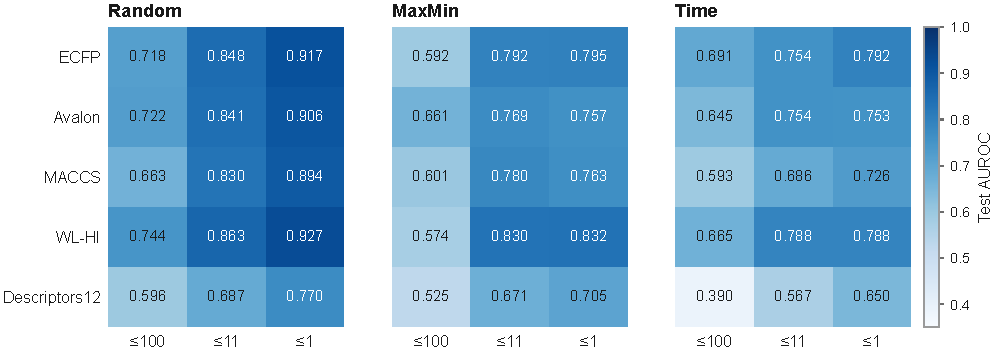
\includegraphics[width=\linewidth]{FigS1_full_performance.pdf}
\caption{\textbf{Full representation-level AUROC matrix.} Each row is one representation--split combination and each column is one nested toxicity endpoint. The \(\leq100~\ugbee\) endpoint is lower than both severe endpoints in all 15 rows.}
\end{figure}

\begin{figure}[H]
\centering
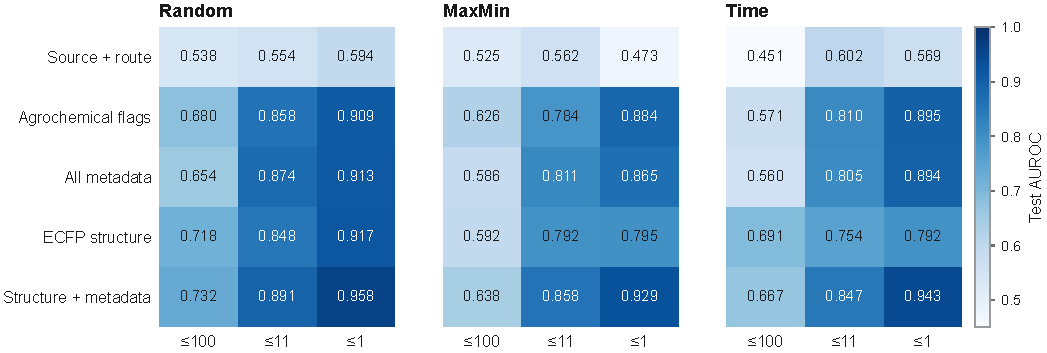
\includegraphics[width=\linewidth]{FigS2_model_decomposition.pdf}
\caption{\textbf{Full model-decomposition AUROC matrix.} Severe-endpoint discrimination is high for agrochemical-use and all-metadata models, while structure-plus-metadata fusion is descriptively strongest in most settings. Incremental-value contrasts and their within-endpoint/split simultaneous bootstrap intervals are printed in Supplementary Table~S5.}
\end{figure}

\begin{figure}[H]
\centering
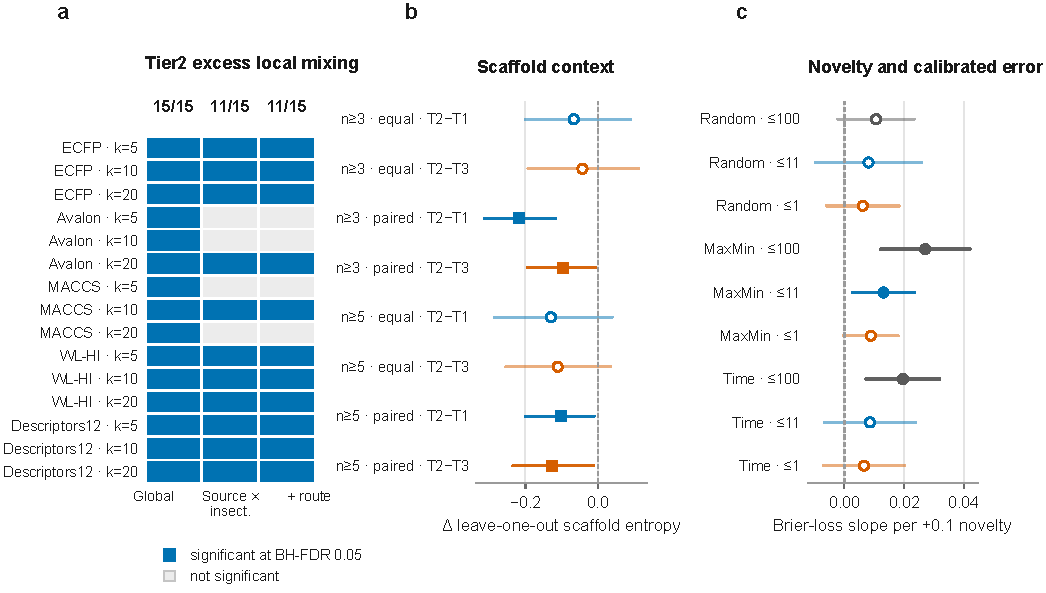
\includegraphics[width=\linewidth]{FigS3_structural_diagnostics.pdf}
\caption{\textbf{Secondary structural diagnostics.} \textbf{(a)} Tier2 excess local mixing: filled cells mark representation-by-$k$ tests significant at BH-FDR 0.05 within each of the global and two composition-conditional null families. \textbf{(b)} Leave-one-out scaffold-context contrasts at minimum scaffold sizes of three and five; circles are scaffold-equal and squares shared-scaffold paired comparisons. These weighting schemes estimate different summaries. \textbf{(c)} Endpoint-specific Brier-loss slope per 0.1 increase in chemical novelty. Filled markers denote marginal slope intervals excluding zero; endpoint interaction tests are reported separately in Supplementary Table~S21c.}
\end{figure}

\begin{figure}[H]
\centering
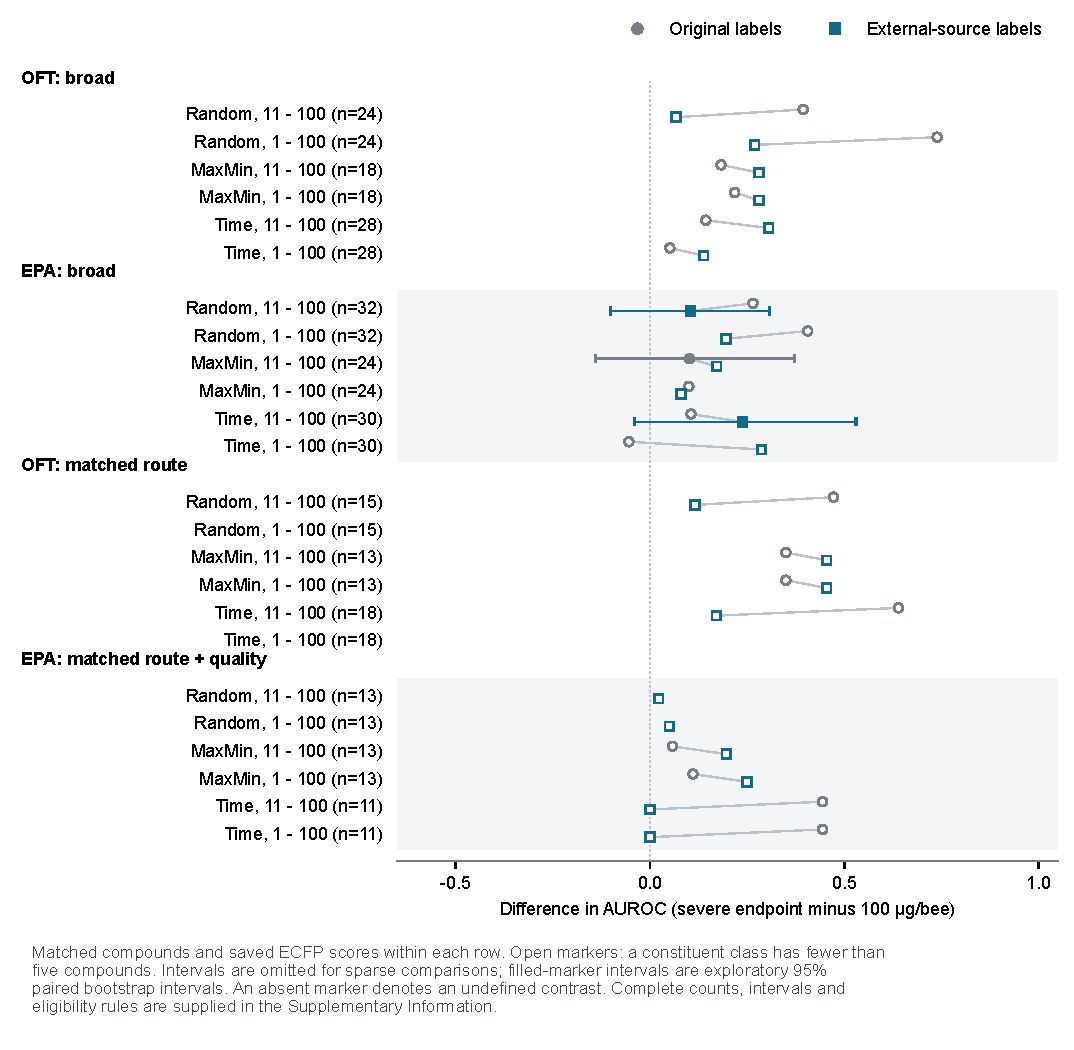
\includegraphics[width=\linewidth]{FigS4_label_source_contrasts.pdf}
\caption{\textbf{Label-source reassessment of paired endpoint contrasts.} Grey circles use original labels and blue squares use source-derived labels on the same compounds and saved ECFP scores. Bars are paired-compound 95\% percentile intervals. Open markers indicate a constituent class below five compounds, for which the interval is omitted; absent markers indicate undefined contrasts. Broad cohorts use external contact endpoints; matched-route and quality screens are defined in the main Methods. Supplementary Table~S18a gives class counts and screens; S18b gives contrast intervals and the CSV location of valid/degenerate-draw counts.}
\end{figure}

\renewcommand{\refname}{Supplementary methodological references}
\begin{thebibliography}{2}
\bibitem{SiLiang1986} K.-Y. Liang and S. L. Zeger, ``Longitudinal data analysis using generalized linear models,'' \textit{Biometrika}, vol. 73, no. 1, pp. 13--22, 1986. \url{https://doi.org/10.1093/biomet/73.1.13}.
\bibitem{SiZou2005} H. Zou and T. Hastie, ``Regularization and variable selection via the elastic net,'' \textit{Journal of the Royal Statistical Society: Series B}, vol. 67, no. 2, pp. 301--320, 2005. \mbox{\url{https://doi.org/10.1111/j.1467-9868.2005.00503.x}}.
\end{thebibliography}

\end{document}
